\documentclass{beamer}

\usepackage[utf8]{inputenc}
\usepackage{booktabs}
\usepackage{xcolor}
%\usetheme{Hannover}
\usecolortheme{crane}
\usepackage{siunitx,cancel}
\usepackage{graphicx}
\usepackage{hyperref}

\usepackage{listings}
\usepackage{color}
\usepackage{xcolor}

%\usepackage[
%backend=biber,
%style=numeric,
%citestyle=numeric,
%sorting=none
%]{biblatex}
%\addbibresource{resources.bib}


% This is the color used for MATLAB comments below
\definecolor{MyDarkGreen}{rgb}{0.0,0.4,0.0}
\definecolor{Blue}{rgb}{0.0,0.0,1.0}
\definecolor{Purple}{rgb}{1.0,0.0,1.0}

\colorlet{mygray}{black!30}
\colorlet{mygreen}{green!60!blue}
\colorlet{mymauve}{red!60!blue}

\lstset{
  backgroundcolor=\color{gray!10},
  basicstyle=\ttfamily,
  columns=fullflexible,
  breakatwhitespace=false,
  breaklines=true,
  captionpos=b,
  commentstyle=\color{mygreen},
  extendedchars=true,
  frame=single,
  keepspaces=true,
  keywordstyle=\color{blue},
  language=c++,
  numbers=none,
  numbersep=5pt,
  numberstyle=\tiny\color{blue},
  rulecolor=\color{mygray},
  showspaces=false,
  showtabs=false,
  stepnumber=5,
  stringstyle=\color{mymauve},
  tabsize=3,
  title=\lstname
}






%\defaultfontfeatures{Scale=MatchLowercase,Mapping=tex-text}
%\setmainfont[Numbers=Lowercase]{Minion Pro}
%\setsansfont[Numbers=Lowercase]{Myriad Pro}
%\setmonofont{Menlo}
%\setmathsfont(Digits,Latin,Greek)[Numbers={Lining,Proportional}]{Minion Pro}

\sisetup{%
  output-decimal-marker = {,},
  per-mode = symbol,
  %round-mode = places,
  %round-precision = 5
}

\DeclareSIUnit \electronvolt {\ensuremath{eV}}
\DeclareSIUnit \lightspeed {\ensuremath{c}}
\DeclareSIUnit \dalton{\ensuremath{u}}
\DeclareSIUnit \echarge{\ensuremath{e}}


\newcommand{\mvec}[2]{
\ensuremath{\left(
\begin{array}{c}
#1\\
#2\\
\end{array}
\right)}
}

\newcommand{\Span}{\ensuremath{\mathrm{Span}}}
\newcommand{\Mat}{\ensuremath{\mathrm{Mat}}}
\newcommand{\R}{\ensuremath{\mathbb{R}}}
\newcommand{\Rno}{\ensuremath{\mathbb{R}\backslash\{0\}}}
\newcommand{\Z}{\ensuremath{\mathbb{Z}}}
\newcommand{\ol}[1]{\ensuremath{\overline{#1} } }
\newcommand{\F}[1]{\ensuremath{\mathbb{F}_{#1} } }


%Information to be included in the title page:
\title{Exploring electric and magnetic forces using computer simulations}
\author{Nikolaj Roager Christensen}
\institute{Student Colloquium in Physics and Astronomy, Aarhus University}
\date{March 2021}

%\AtBeginSection[]
%{
%}

\titlegraphic
{
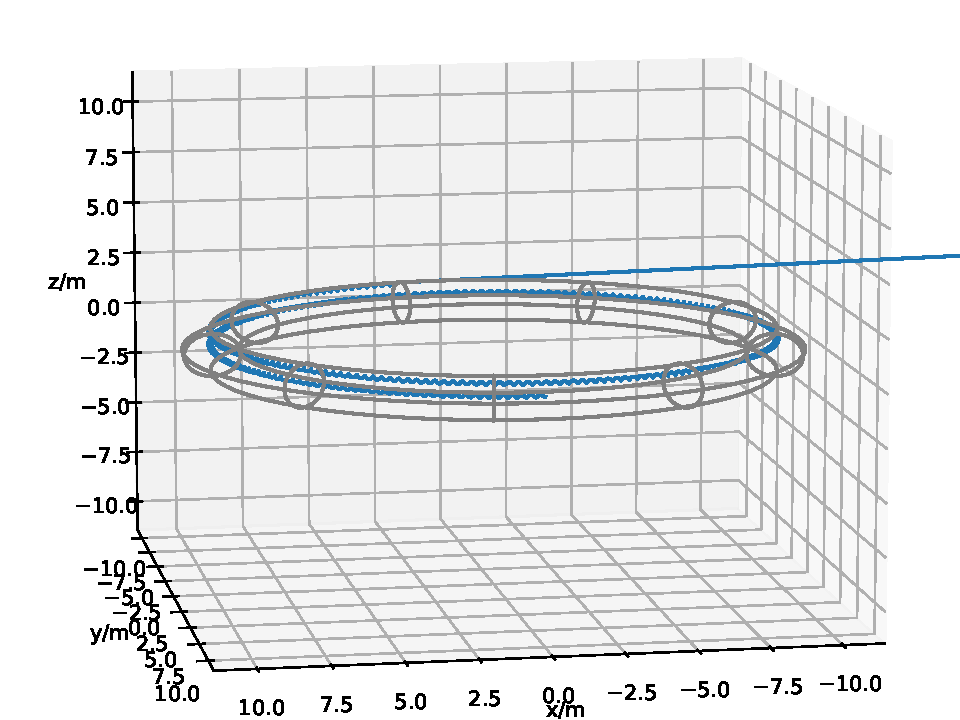
\includegraphics[width=0.5\textwidth]{torus4_3D.pdf}
}
\begin{document}

\frame{\titlepage}



\section{Introduction (3 minutes)}

\begin{frame}
\frametitle{Wellcome}

\begin{itemize}
\item<1-> Todays topic: particles in electric and magnetic fields
\item<2-> Explored using computer-simulations
\item<3-> Todays plan
\end{itemize}

 \visible<3->{%
\tableofcontents
}
\end{frame}


\begin{frame}
\frametitle{Introduction, what and why}
\begin{columns}
\begin{column}{0.5\linewidth}
\begin{itemize}
\item<1-> (Classical) Charged particles in Electric and Magnetic fields
\item<2-> How can magnetic fields steer and collect particles
\item<3-> Real world examples:
\begin{itemize}
\item<3-> Magnetic traps: ``Tokamak" style fusion reactors.
\item<4-> Particle accelerators, here cyclotron.
\item<5-> The Aurora.
\end{itemize}
\end{itemize}
\end{column}
\begin{column}{0.5\linewidth}

\only<2>
{%
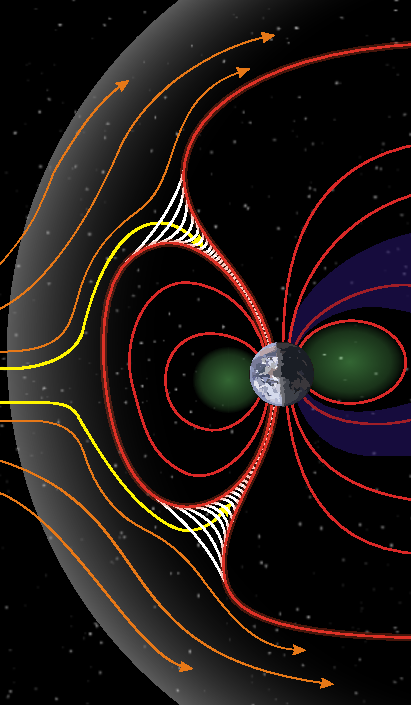
\includegraphics[width=0.8\linewidth]{Structure_of_the_magnetosphere_Nasa.pdf}%
{\color{gray} Illustration originally from Nasa. Published on wikipedia, in Public Domain (Cropped to fit page) }
}%
\only<3>{
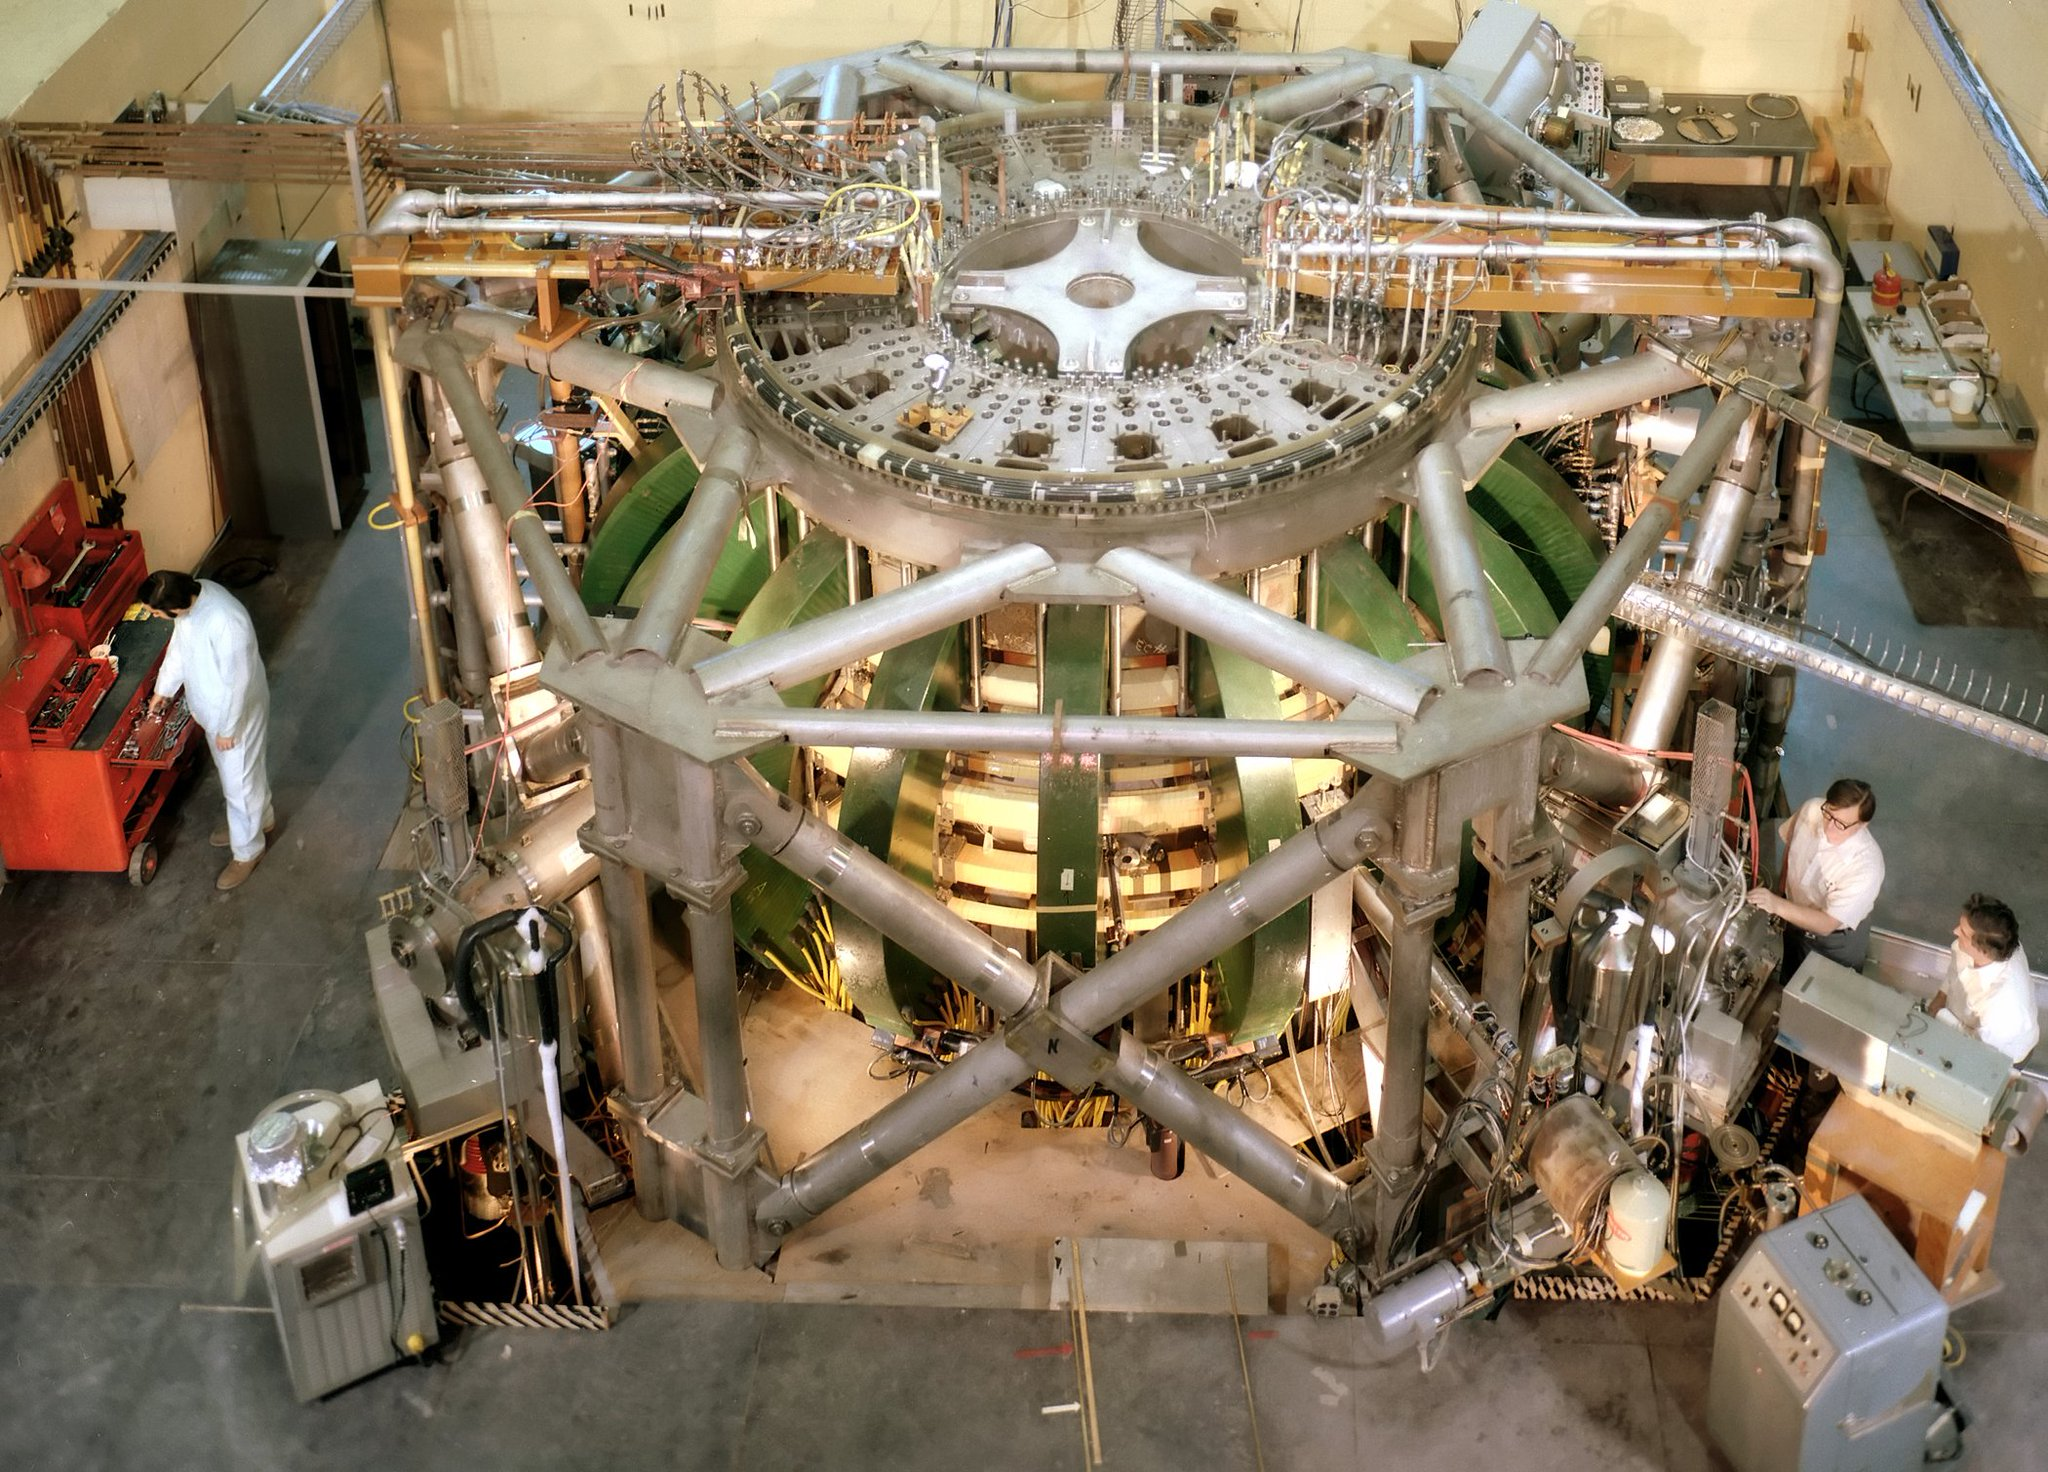
\includegraphics[width=\linewidth]{Princeton_Large_Torus_1975.jpg}

{\color{gray} Princeton Large Torus in 1975, image in Public Domain}
}%
\only<4>{
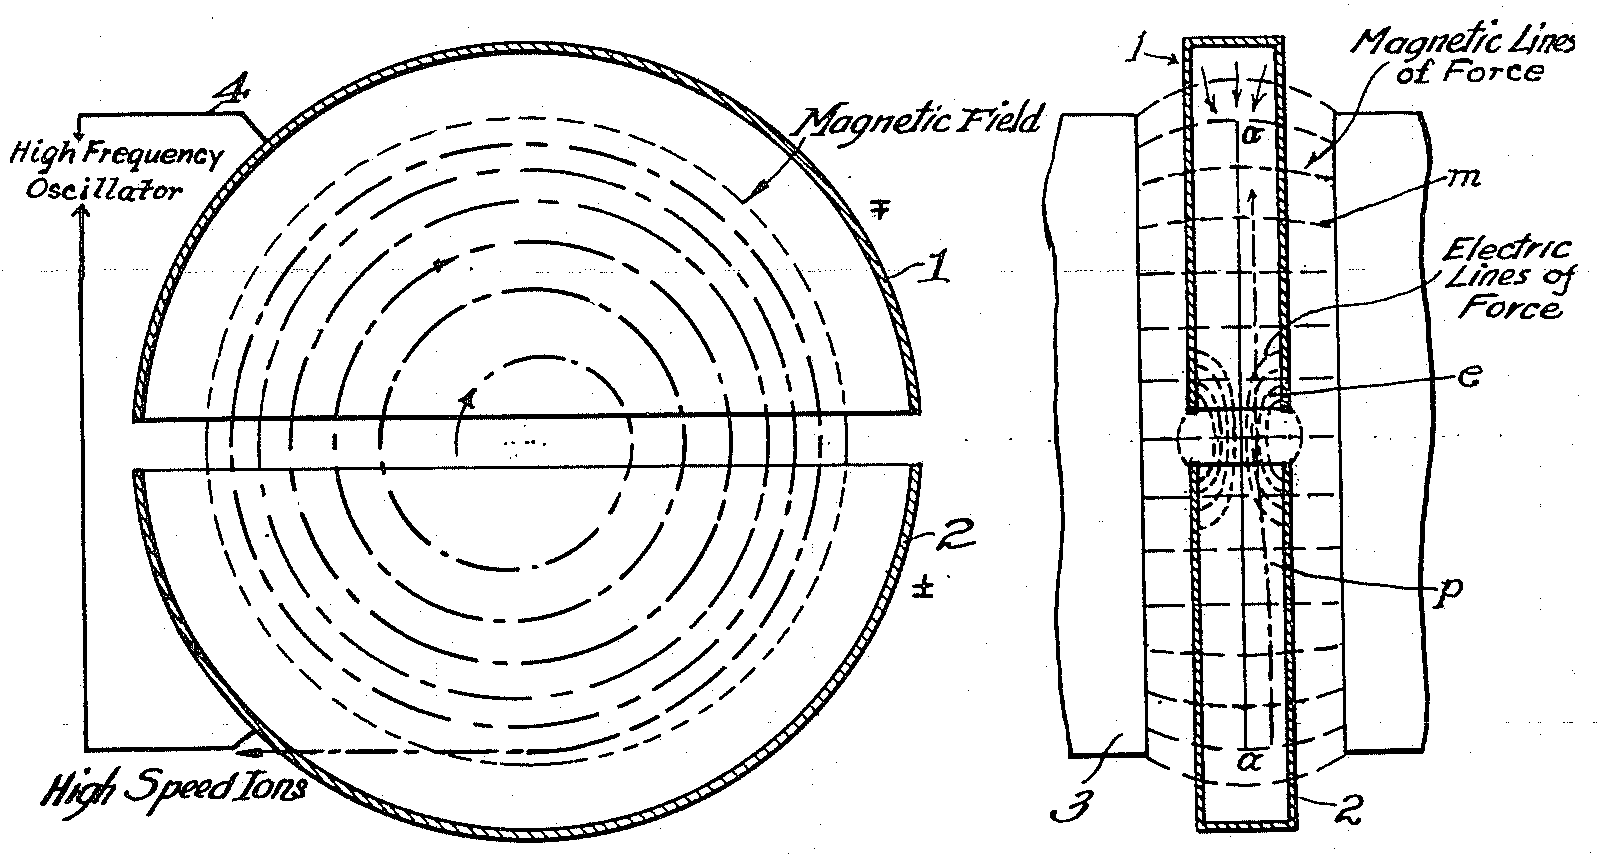
\includegraphics[width=\linewidth]{ Cyclotron_patent.png}


{\color{gray} Ernest O. Lawrence, 1934, U.S. Patent 1,948,384; image in Public Domain}
}%
\only<5>{
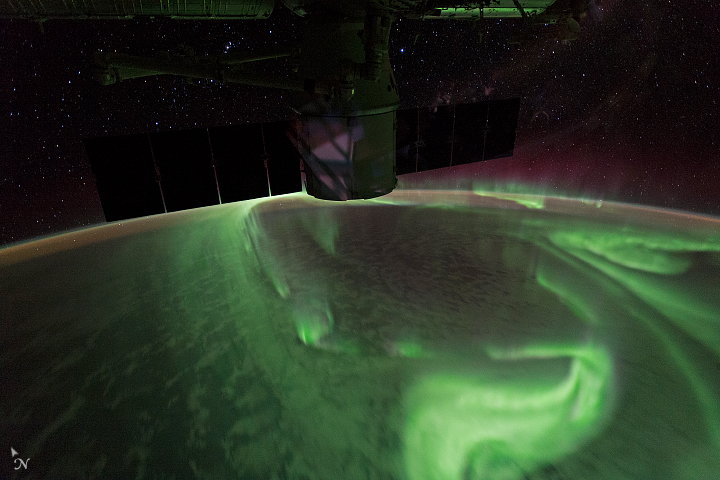
\includegraphics[width=\linewidth]{Aurora_australis_ISS.jpg}

{\color{gray} Nasa: Aurora Australis, Indian Ocean from ISS in 2017; image in Public domain}
}
\end{column}
\end{columns}
\end{frame}


\begin{frame}
\frametitle{How: Numeric-simulation}
\begin{itemize}
\item<1-> When analytical solutions are not practical.
\item<2-> Testing experimental setups.
\item<4-> Here, the \lstinline{odeint} library in C++.
\begin{itemize}
\item<4-> Runge Kutta Algorithm
\item<4-> Identical to \lstinline{odeint}/\lstinline{ode45} in scipy or matlab.
\end{itemize}
\item<3-> Not the main focus.
\item<5-> Simulations are not experiments!
\end{itemize}
\end{frame}

\section{Theory and background (13 minutes)}

\begin{frame}
\frametitle{Theory and background (13 minutes)}
\tableofcontents[currentsection]
\end{frame}



\begin{frame}
\frametitle{Theory: Electric and magnetic fields}
\begin{itemize}
\item<1-> Some repetition from Electrodynamics
\item<2-> The Lorentz force:

\begin{equation*}
\vec{F} = q ( \vec{v}\times \vec{B}+\vec{E}).
\end{equation*}


\item<3-> Only 1 particle! so pre-programmed depending on the setup.
\end{itemize}
\end{frame}

\begin{frame}
\begin{itemize}
\frametitle{Theory: Alternative approach}

\item<1-> I used:

\begin{align*}
m \ddot{\vec{r}} &= q ( \dot{\vec{r}}\times \vec{B}+\vec{E}).
\end{align*}

\item<2-> Other options exists: potentials

\begin{align*}
\vec{E}(\vec{r},t) &= \nabla \phi(\vec{r},t)\\
\vec{B}(\vec{r},t) &= \nabla \times \vec{A}(\vec{r},t)
\end{align*}

\item<3-> Hamiltonian equation of motion

\begin{align*}
\dot{r_i} &= \frac{\partial \mathcal{H}}{\partial p_i},\\
\mathcal{H} &= \frac{\vec{p}^2}{2m}+V(\vec{r}) \rightarrow \frac{(\vec{p}^2-q\vec{A}(\vec{r},t))}{2m}+q\phi(\vec{r},t)+V(\vec{r}).
\end{align*}

\end{itemize}
\end{frame}

\newif\ifadditional
%\additionalfalse
\additionaltrue

\ifadditional
\begin{frame}[fragile]
\frametitle{The ODE implementation}
%\only<1>{%
\begin{lstlisting}
auto ODE = [...](const state_type Data, state_type &dDatadt, const double t)
{
    //Extract position and velocity from data
    ...

    //Get current force
    vec F = Charge*(Fields.get_Efield(pos,t)+
        cross(velocity,Fields.get_Bfield(pos,t)));

    vec dVdt = F*Inv_mass;  //get acceleration

    //Save derivative of data
    ...
};
\end{lstlisting}
\end{frame}
\fi

\begin{frame}
\frametitle{Known results, cyclotron motion $\vec{B}$ fields}
\begin{columns}
\begin{column}{0.5\linewidth}
\begin{itemize}
\item<2-> Magnetic forces do no work:

\begin{equation*}
dW_{\vec{B}}= \vec{F}_B \cdot d\vec{r}\propto (\vec{v}\times \vec{B})\cdot \vec{v} = 0.
\end{equation*}

\item<3-> ($\vec{v}=\vec{v}_\perp+\vec{v}_\parallel$):

\begin{equation*}
|\vec{F}_B| = |q ( \vec{v}\times \vec{B})| =|q v_{\perp} B|.
\end{equation*}
\item<4-> Same as Centripetal force: Cyclotron motion

\item<5-> Cyclotron radius and frequency:

\begin{equation*}
R = \frac{v_\perp m}{|q|B} \quad \omega_c =\frac{|q|B}{m}.
\end{equation*}

\end{itemize}
\end{column}
\begin{column}{0.5\linewidth}
\only<1-2>{%
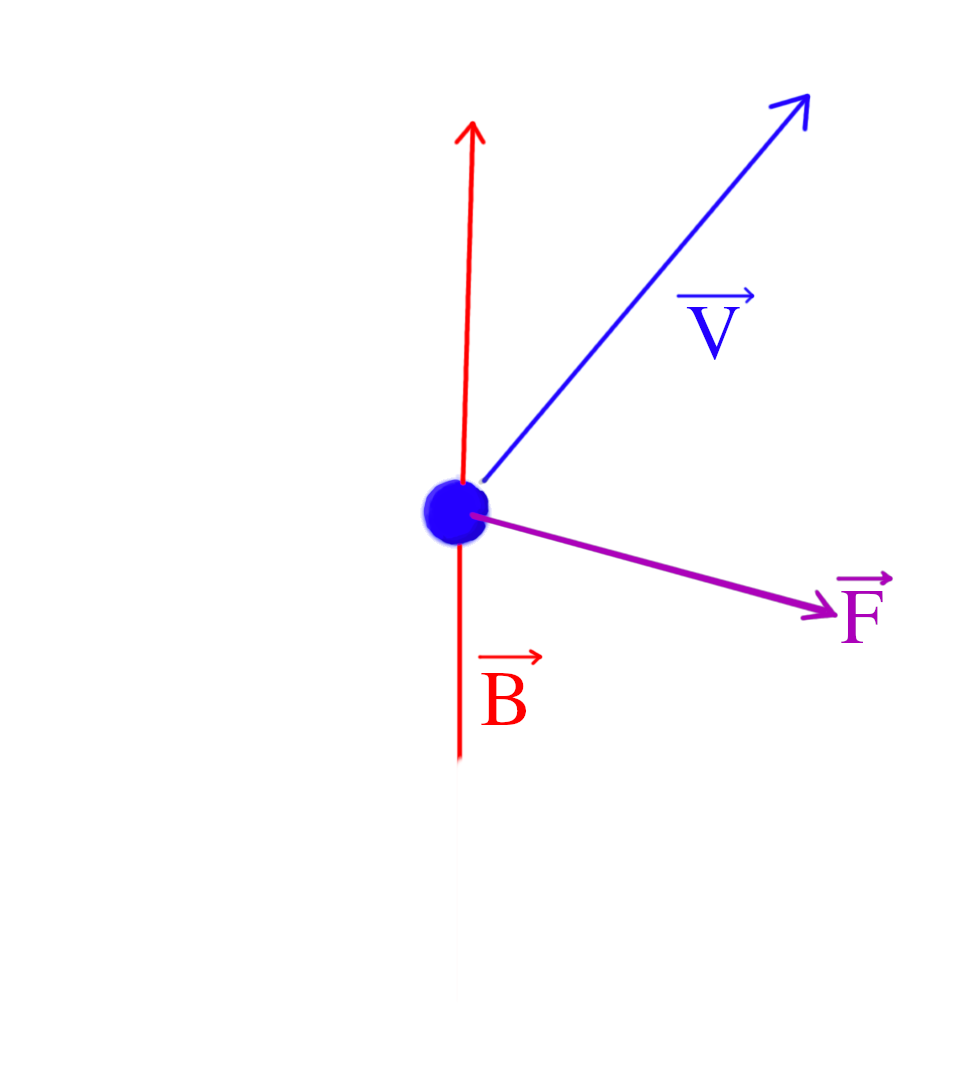
\includegraphics[width=\linewidth]{dw0.png}}%
\only<3->{%
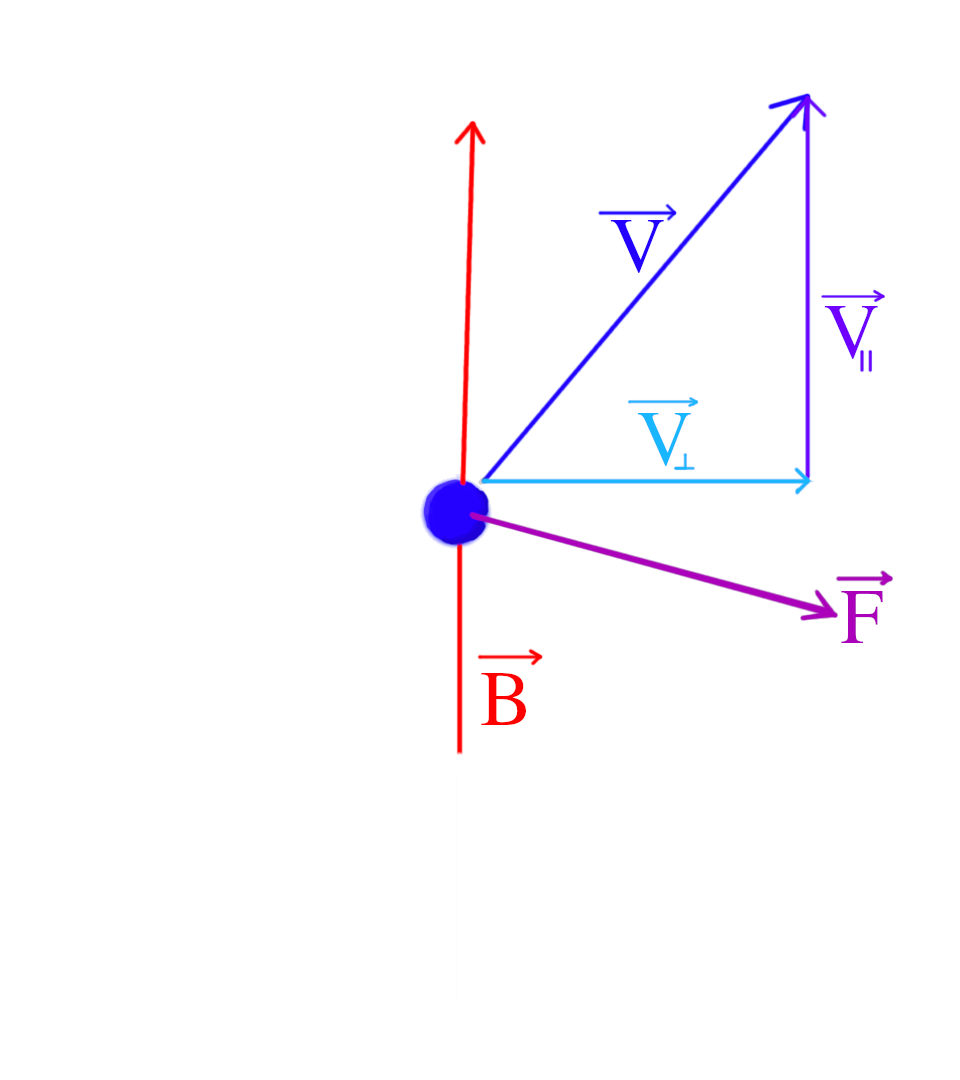
\includegraphics[width=\linewidth]{cyc0.png}}%
%\only<4->{%
%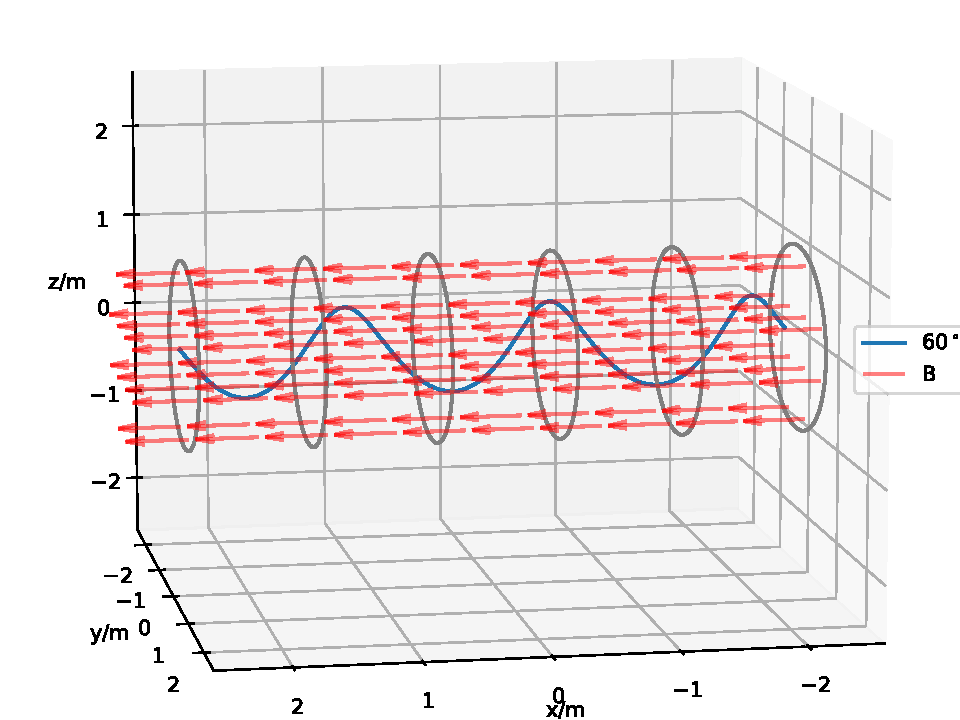
\includegraphics[width=\linewidth]{helix.pdf}}%
\end{column}
\end{columns}
\end{frame}





\begin{frame}
\frametitle{Protons in a Solenoid, 3D plots}
\only<1>{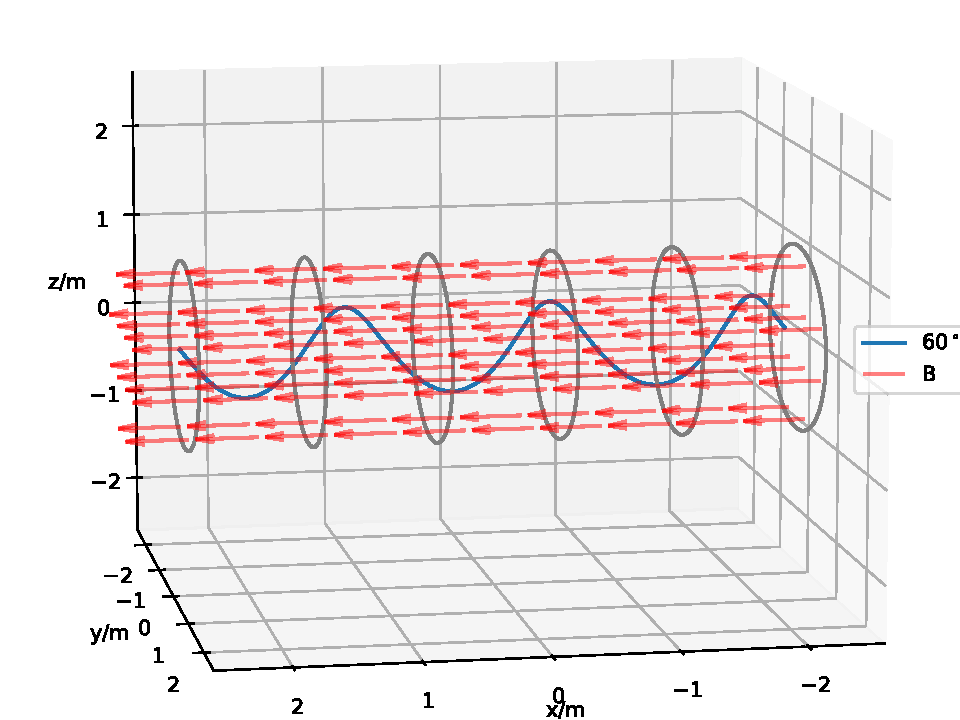
\includegraphics[width=0.8\linewidth]{helix.pdf}}%
\only<2>{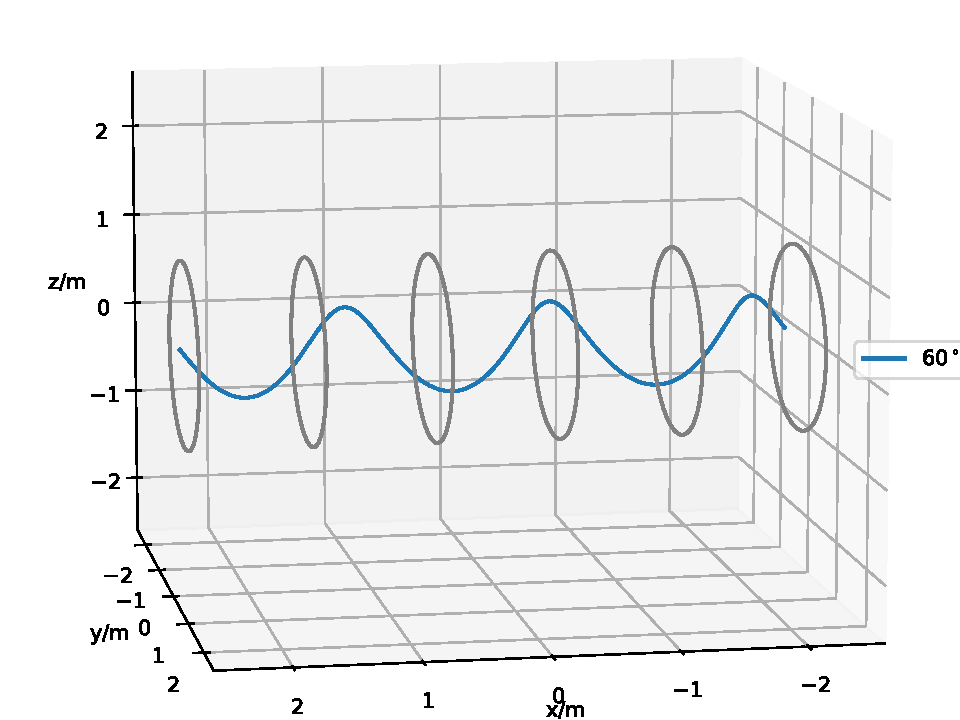
\includegraphics[width=0.8\linewidth]{helix1.pdf}}%
\only<3>{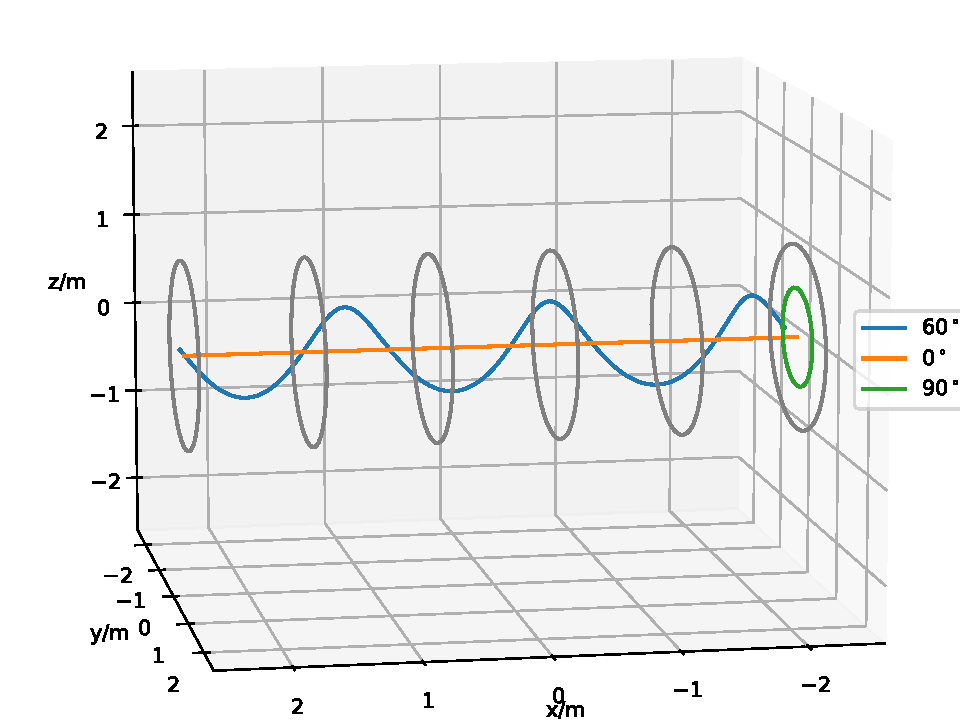
\includegraphics[width=0.8\linewidth]{solenoid_3D0.pdf}}%
\only<4>{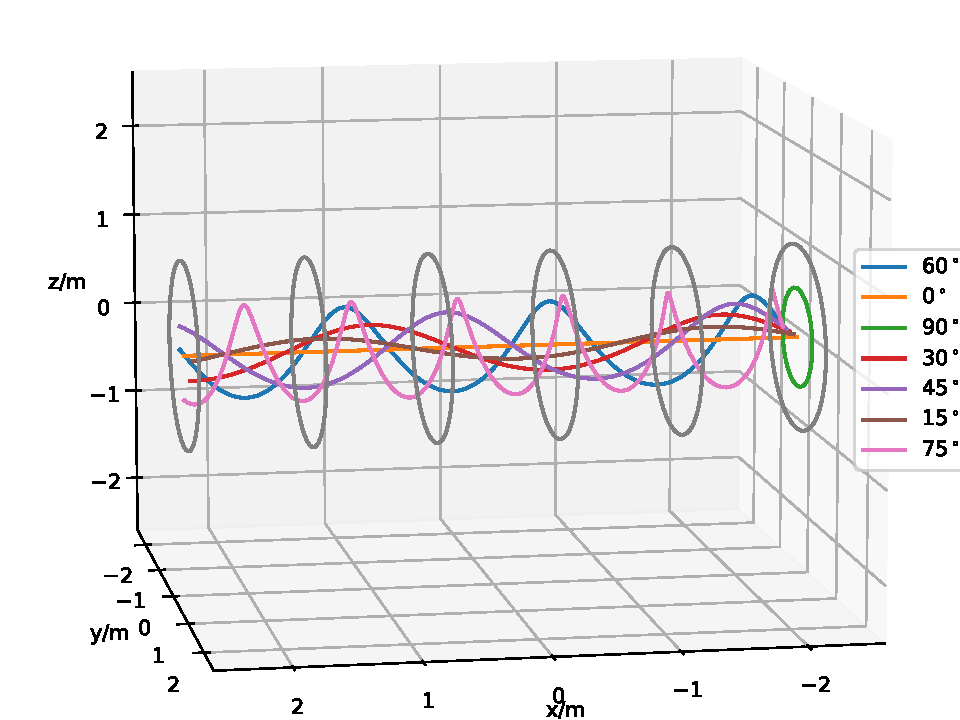
\includegraphics[width=0.8\linewidth]{solenoid_3D1.pdf}}%


\begin{itemize}
\item<1> Solenoid with $N=1000$ turns per $m$, $I=\SI{5}{\ampere}$, $r=\SI{1}{\meter}$, $|\vec{B}|\approx\SI{6}{\milli\tesla}$.
\item<1> Proton with $E_{kin}=\SI{1}{\mega\electronvolt\per\square\lightspeed}$ ($|v|\approx \SI{3.195E5}{\meter\per\second}$)
\end{itemize}

\end{frame}


\begin{frame}
\frametitle{Protons in a Solenoid, 2D plots}
\only<1>{%
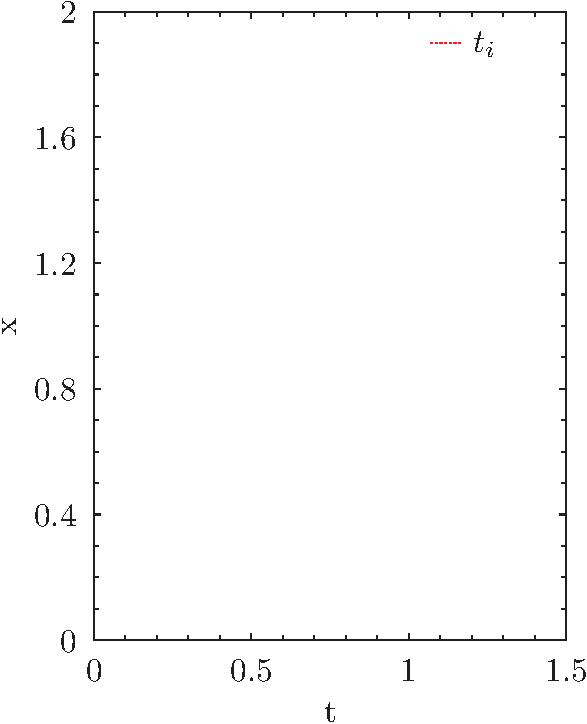
\includegraphics[width=0.66\linewidth]{solenoid_xz_view1.pdf}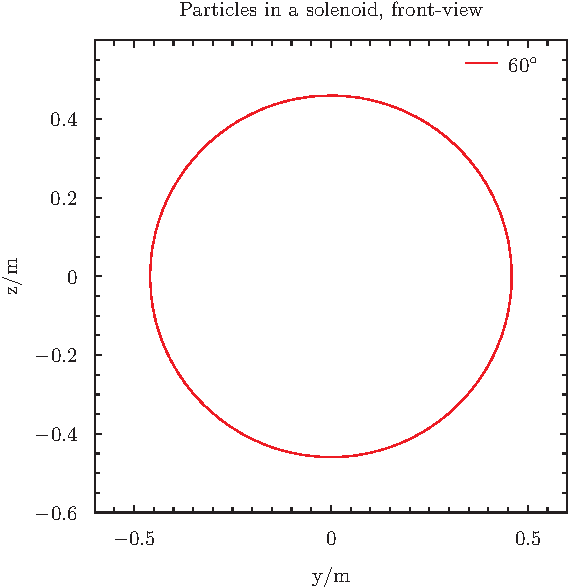
\includegraphics[width=0.33\linewidth]{solenoid_yz_view1.pdf}}%
\only<2>{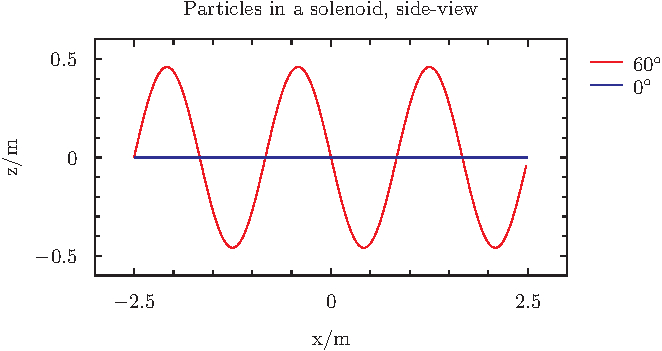
\includegraphics[width=0.66\linewidth]{solenoid_xz_view2.pdf}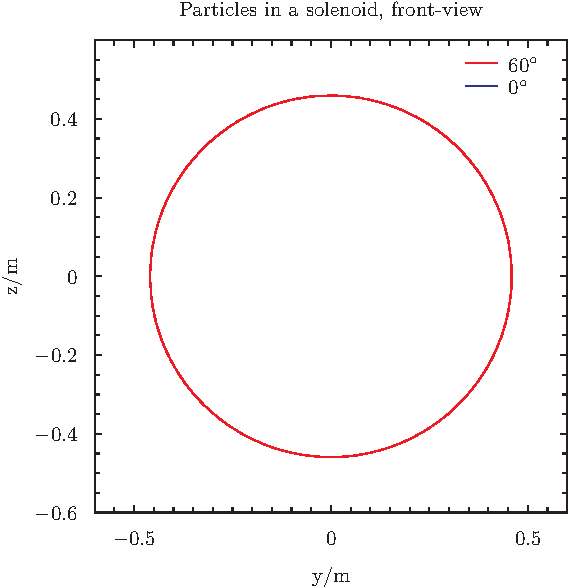
\includegraphics[width=0.33\linewidth]{solenoid_yz_view2.pdf}}%
\only<3>{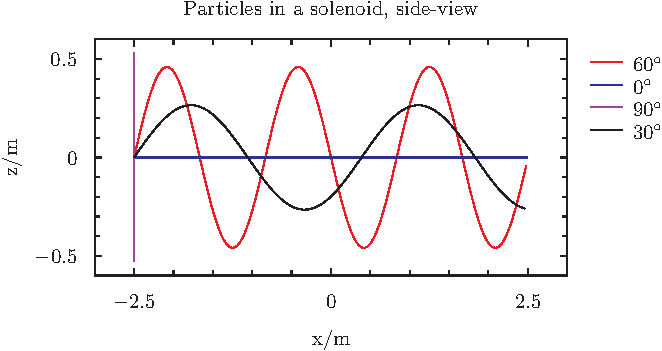
\includegraphics[width=0.66\linewidth]{solenoid_xz_view3.pdf}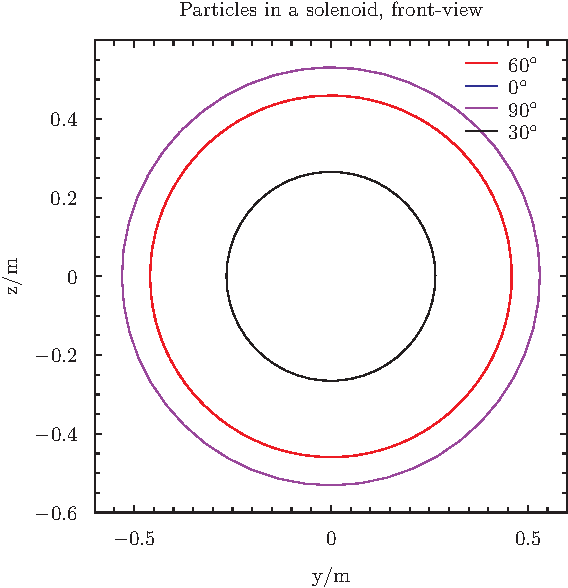
\includegraphics[width=0.33\linewidth]{solenoid_yz_view3.pdf}}%
\only<4>{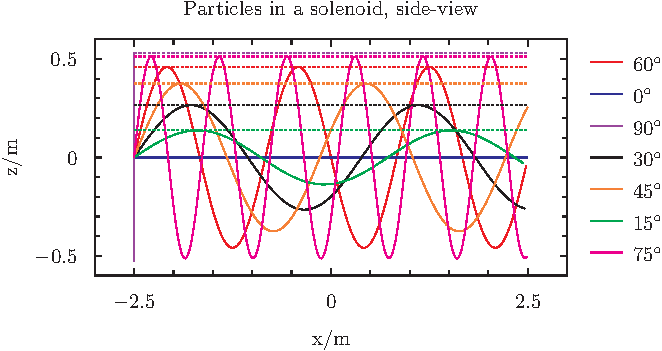
\includegraphics[width=0.66\linewidth]{solenoid_xz_view4.pdf}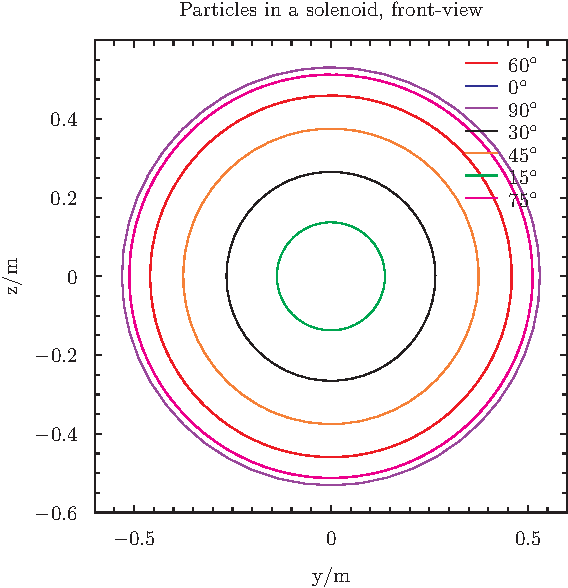
\includegraphics[width=0.33\linewidth]{solenoid_yz_view4.pdf}}%
\only<5>{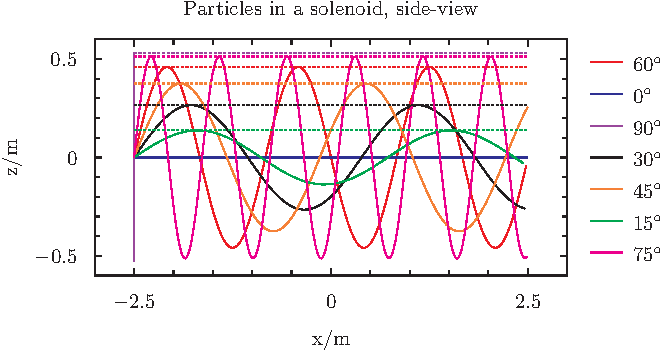
\includegraphics[width=\linewidth]{solenoid_xz_view5.pdf}}%
\only<6>{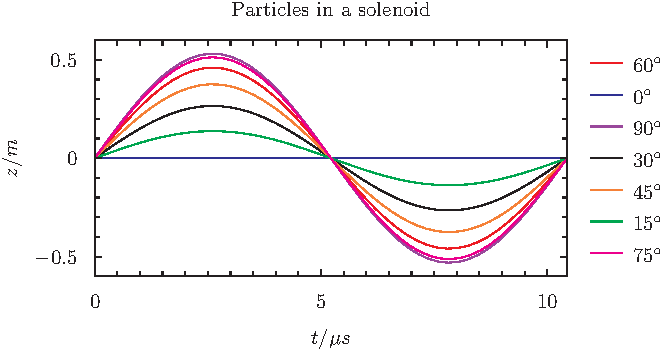
\includegraphics[width=\linewidth]{solenoid_tz.pdf}}

\only<5->{
\begin{equation*}
R \approx \SI{0.5}{\meter}\sin(\theta) \quad T=\frac{2\pi}{\omega_c} \approx \SI{10}{\micro\second}
\end{equation*}
}
\end{frame}

\begin{frame}
\frametitle{Sanity check, no work}
\only<1>{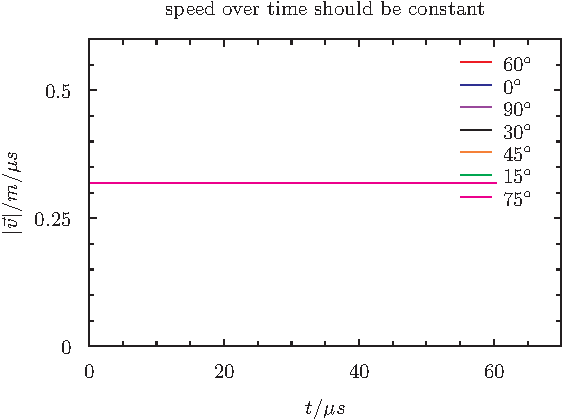
\includegraphics[width=\linewidth]{solenoid_speed1.pdf}}%
\only<2>{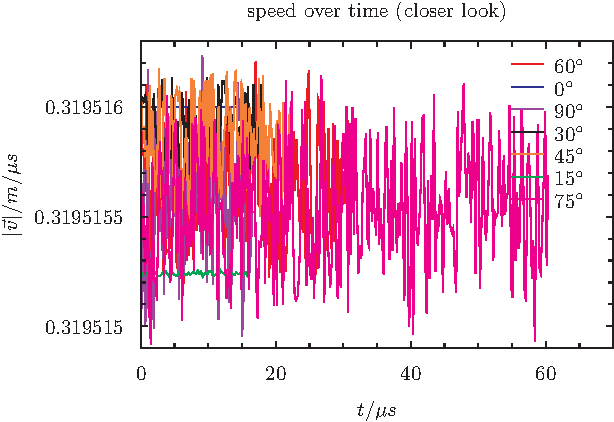
\includegraphics[width=\linewidth]{solenoid_speed2.pdf}}%
\end{frame}


\section{Steering particles with $\vec{B}$ fields (14 min)}

\begin{frame}
\frametitle{Steering particles with $\vec{B}$ fields (14 min)}
\tableofcontents[currentsection]
\end{frame}


\begin{frame}
\frametitle{how can $\vec{B}$ field steer particles}
\begin{columns}
\begin{column}{0.5\linewidth}
\begin{itemize}
\item<1-> The parallel velocity is untouched.

\item<2-> Particles at angle are ``trapped".

\item<3-> What if instead the field curves.

\item<4-> Example torus:

\begin{equation*}
\vec{B}(z,r,\phi)=\vec{\hat{\phi}}\mu_0\frac{N_{tot} I}{2\pi r}=\vec{\hat{\phi}} B(R)\frac{R}{r}.
\end{equation*}

\end{itemize}
\end{column}
\begin{column}{0.5\linewidth}
\only<1-3>{%
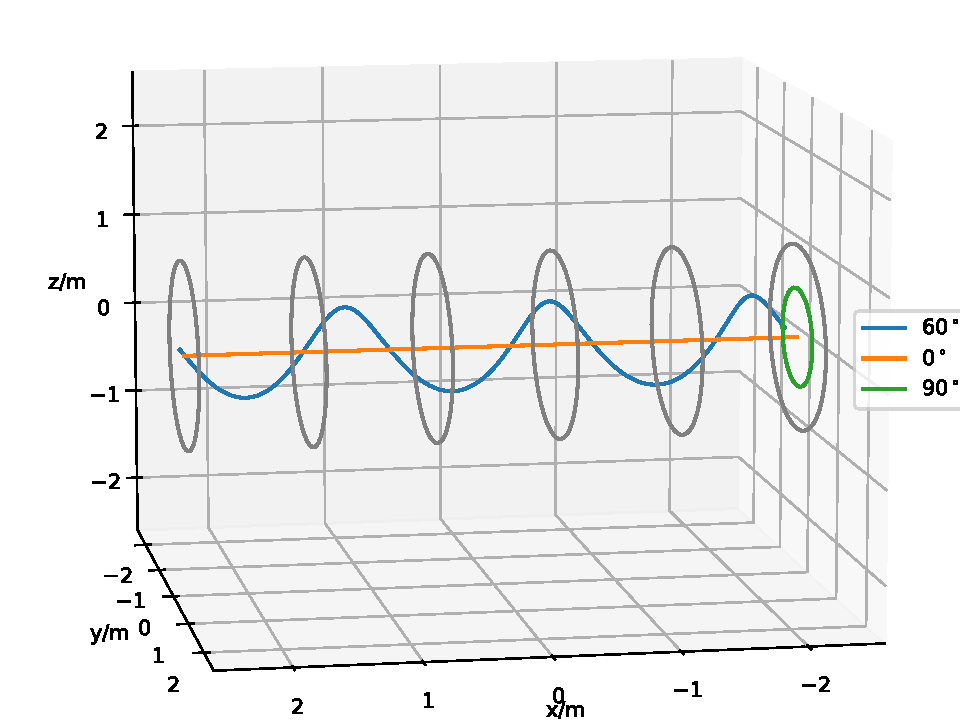
\includegraphics[width=\linewidth]{solenoid_3D0.pdf}}%
\only<4->{%
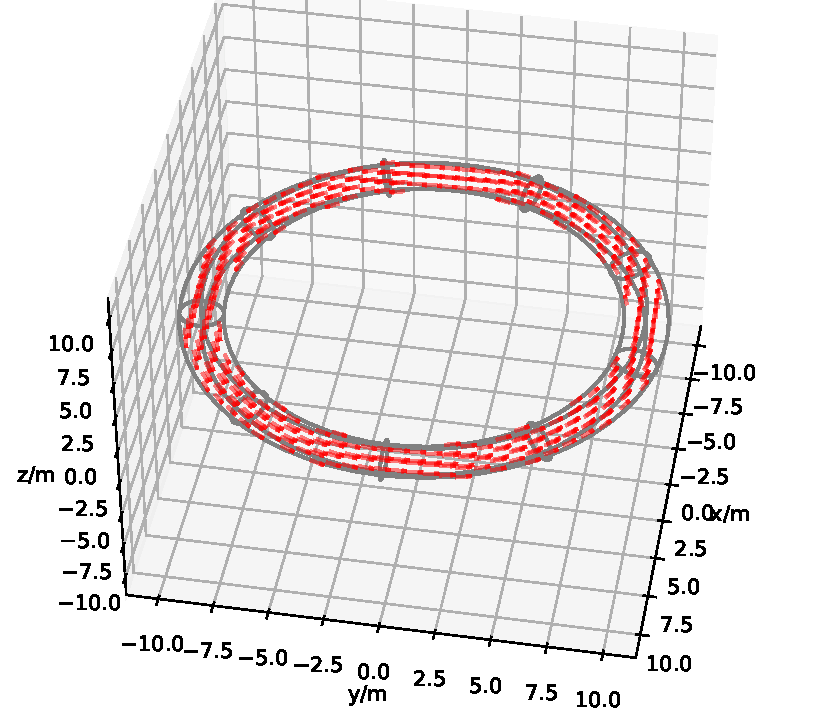
\includegraphics[width=\linewidth]{torus0_3D.pdf}}%
\end{column}
\end{columns}
\end{frame}


\begin{frame}
\frametitle{how can $\vec{B}$ field steer particles}
\only<1>{%
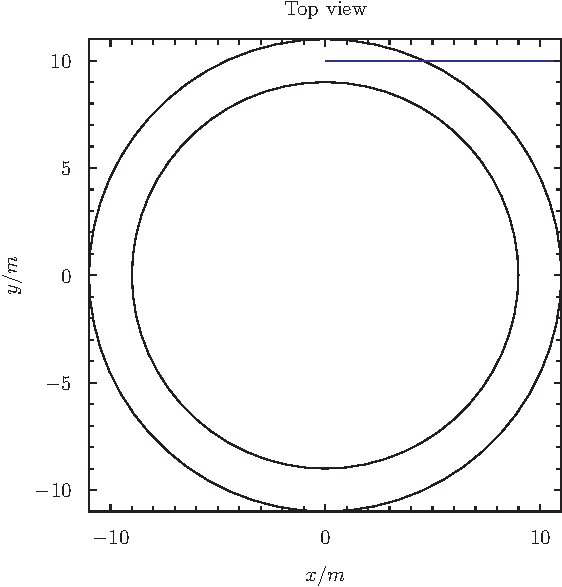
\includegraphics[width=0.7\linewidth]{torus_xyview0.pdf}
}%
\only<2>{%
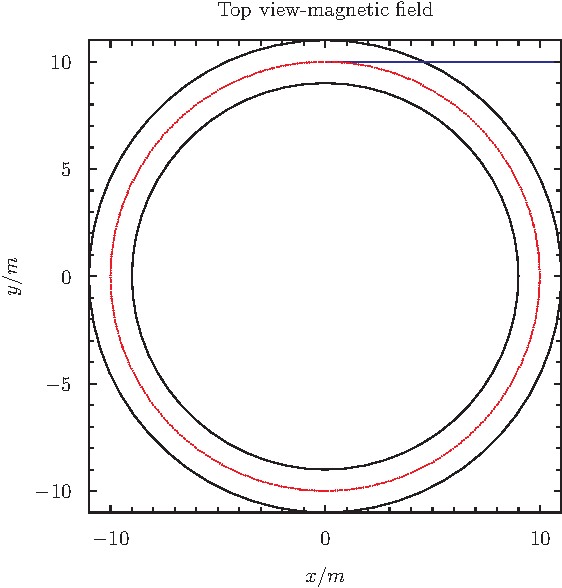
\includegraphics[width=0.7\linewidth]{torus_xyview1.pdf}
}%
\end{frame}


\begin{frame}
\frametitle{Containing protons in a Torus}
\only<1>{%
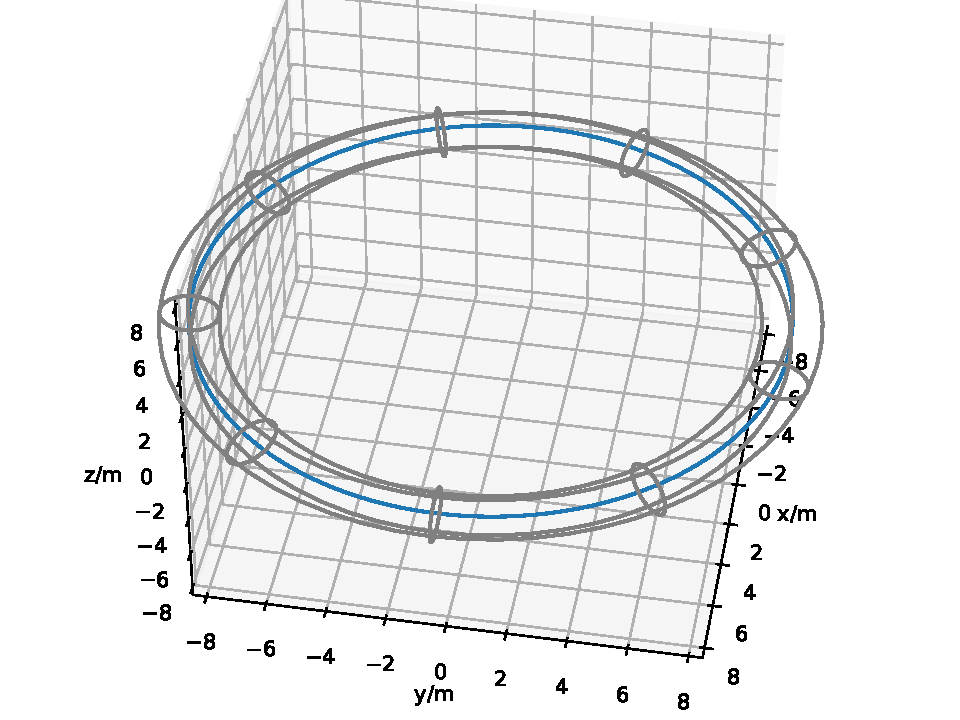
\includegraphics[width=0.8\linewidth]{torus1_3D.pdf}
Proton starting at $(0,10,0)$, $\vec{v}_0=(0.3,0,0) \si{\meter\per\micro\second}$. $|B|\approx \SI{60}{\milli\tesla}$
}%
\only<2>{%
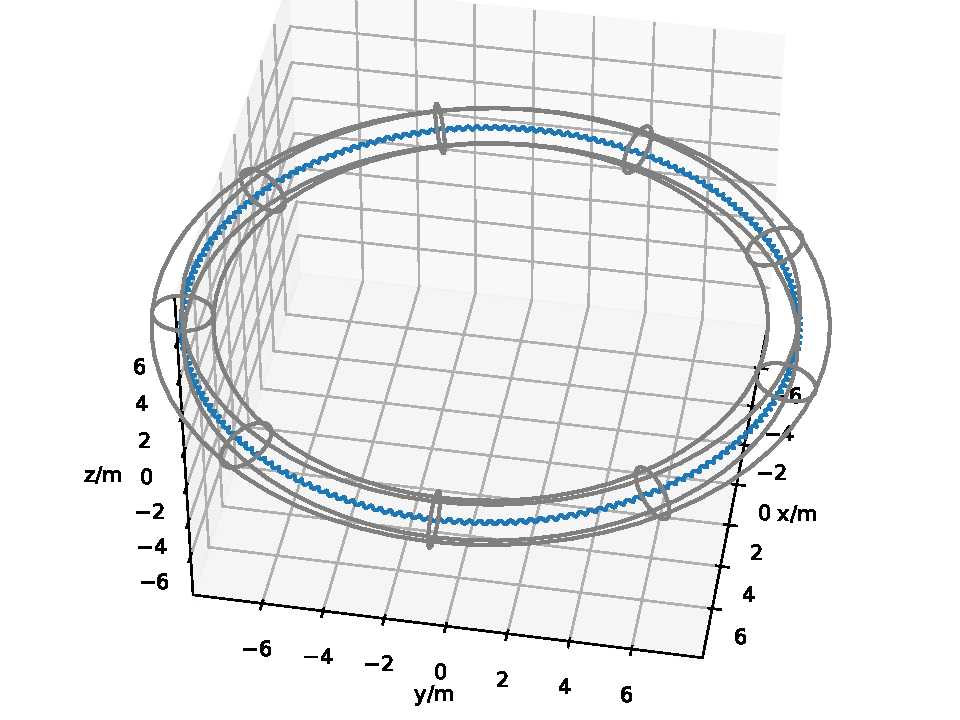
\includegraphics[width=0.8\linewidth]{torus2_3D.pdf}
Proton starting at $(0,10,0)$, $\vec{v}_0=(0.3,0.4,0) \si{\meter\per\micro\second}$.
}%
\end{frame}


\begin{frame}
\frametitle{Instability, Error?}
\only<1>{%
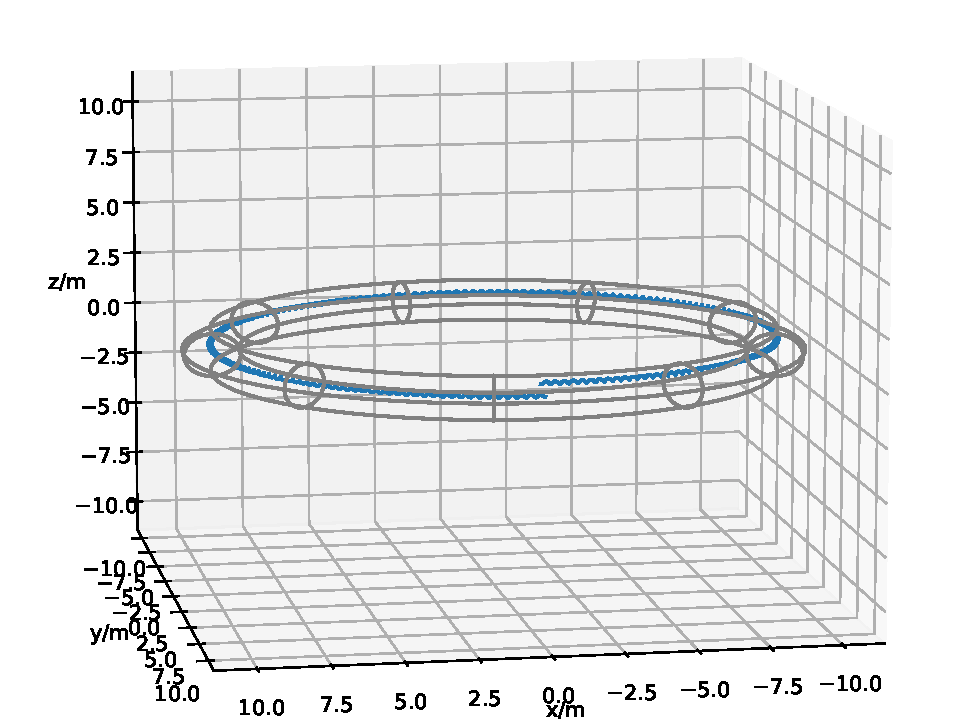
\includegraphics[width=0.8\linewidth]{torus3_3D.pdf}
}%
\only<2>{%
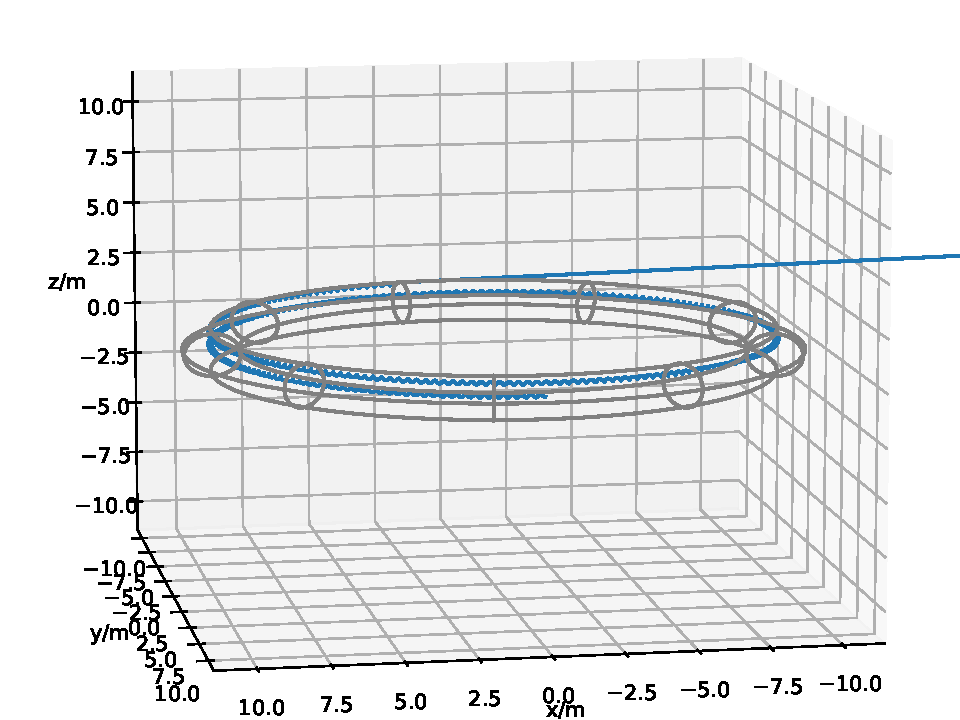
\includegraphics[width=0.8\linewidth]{torus4_3D.pdf}
}%
\end{frame}

\begin{frame}
\frametitle{Not a torus}
\begin{columns}
\begin{column}{0.5\linewidth}
\begin{itemize}
\item<1-> ``Tokamak" style reactors are NOT toruses.

\item<2-> Remember:

\begin{equation*}
\vec{B}(z,r,\phi)=\vec{\hat{\phi}} B(R)\frac{R}{r}.
\end{equation*}

\item<3-> Does lead to drift.

\end{itemize}
\end{column}
\begin{column}{0.5\linewidth}
\only<1>{%
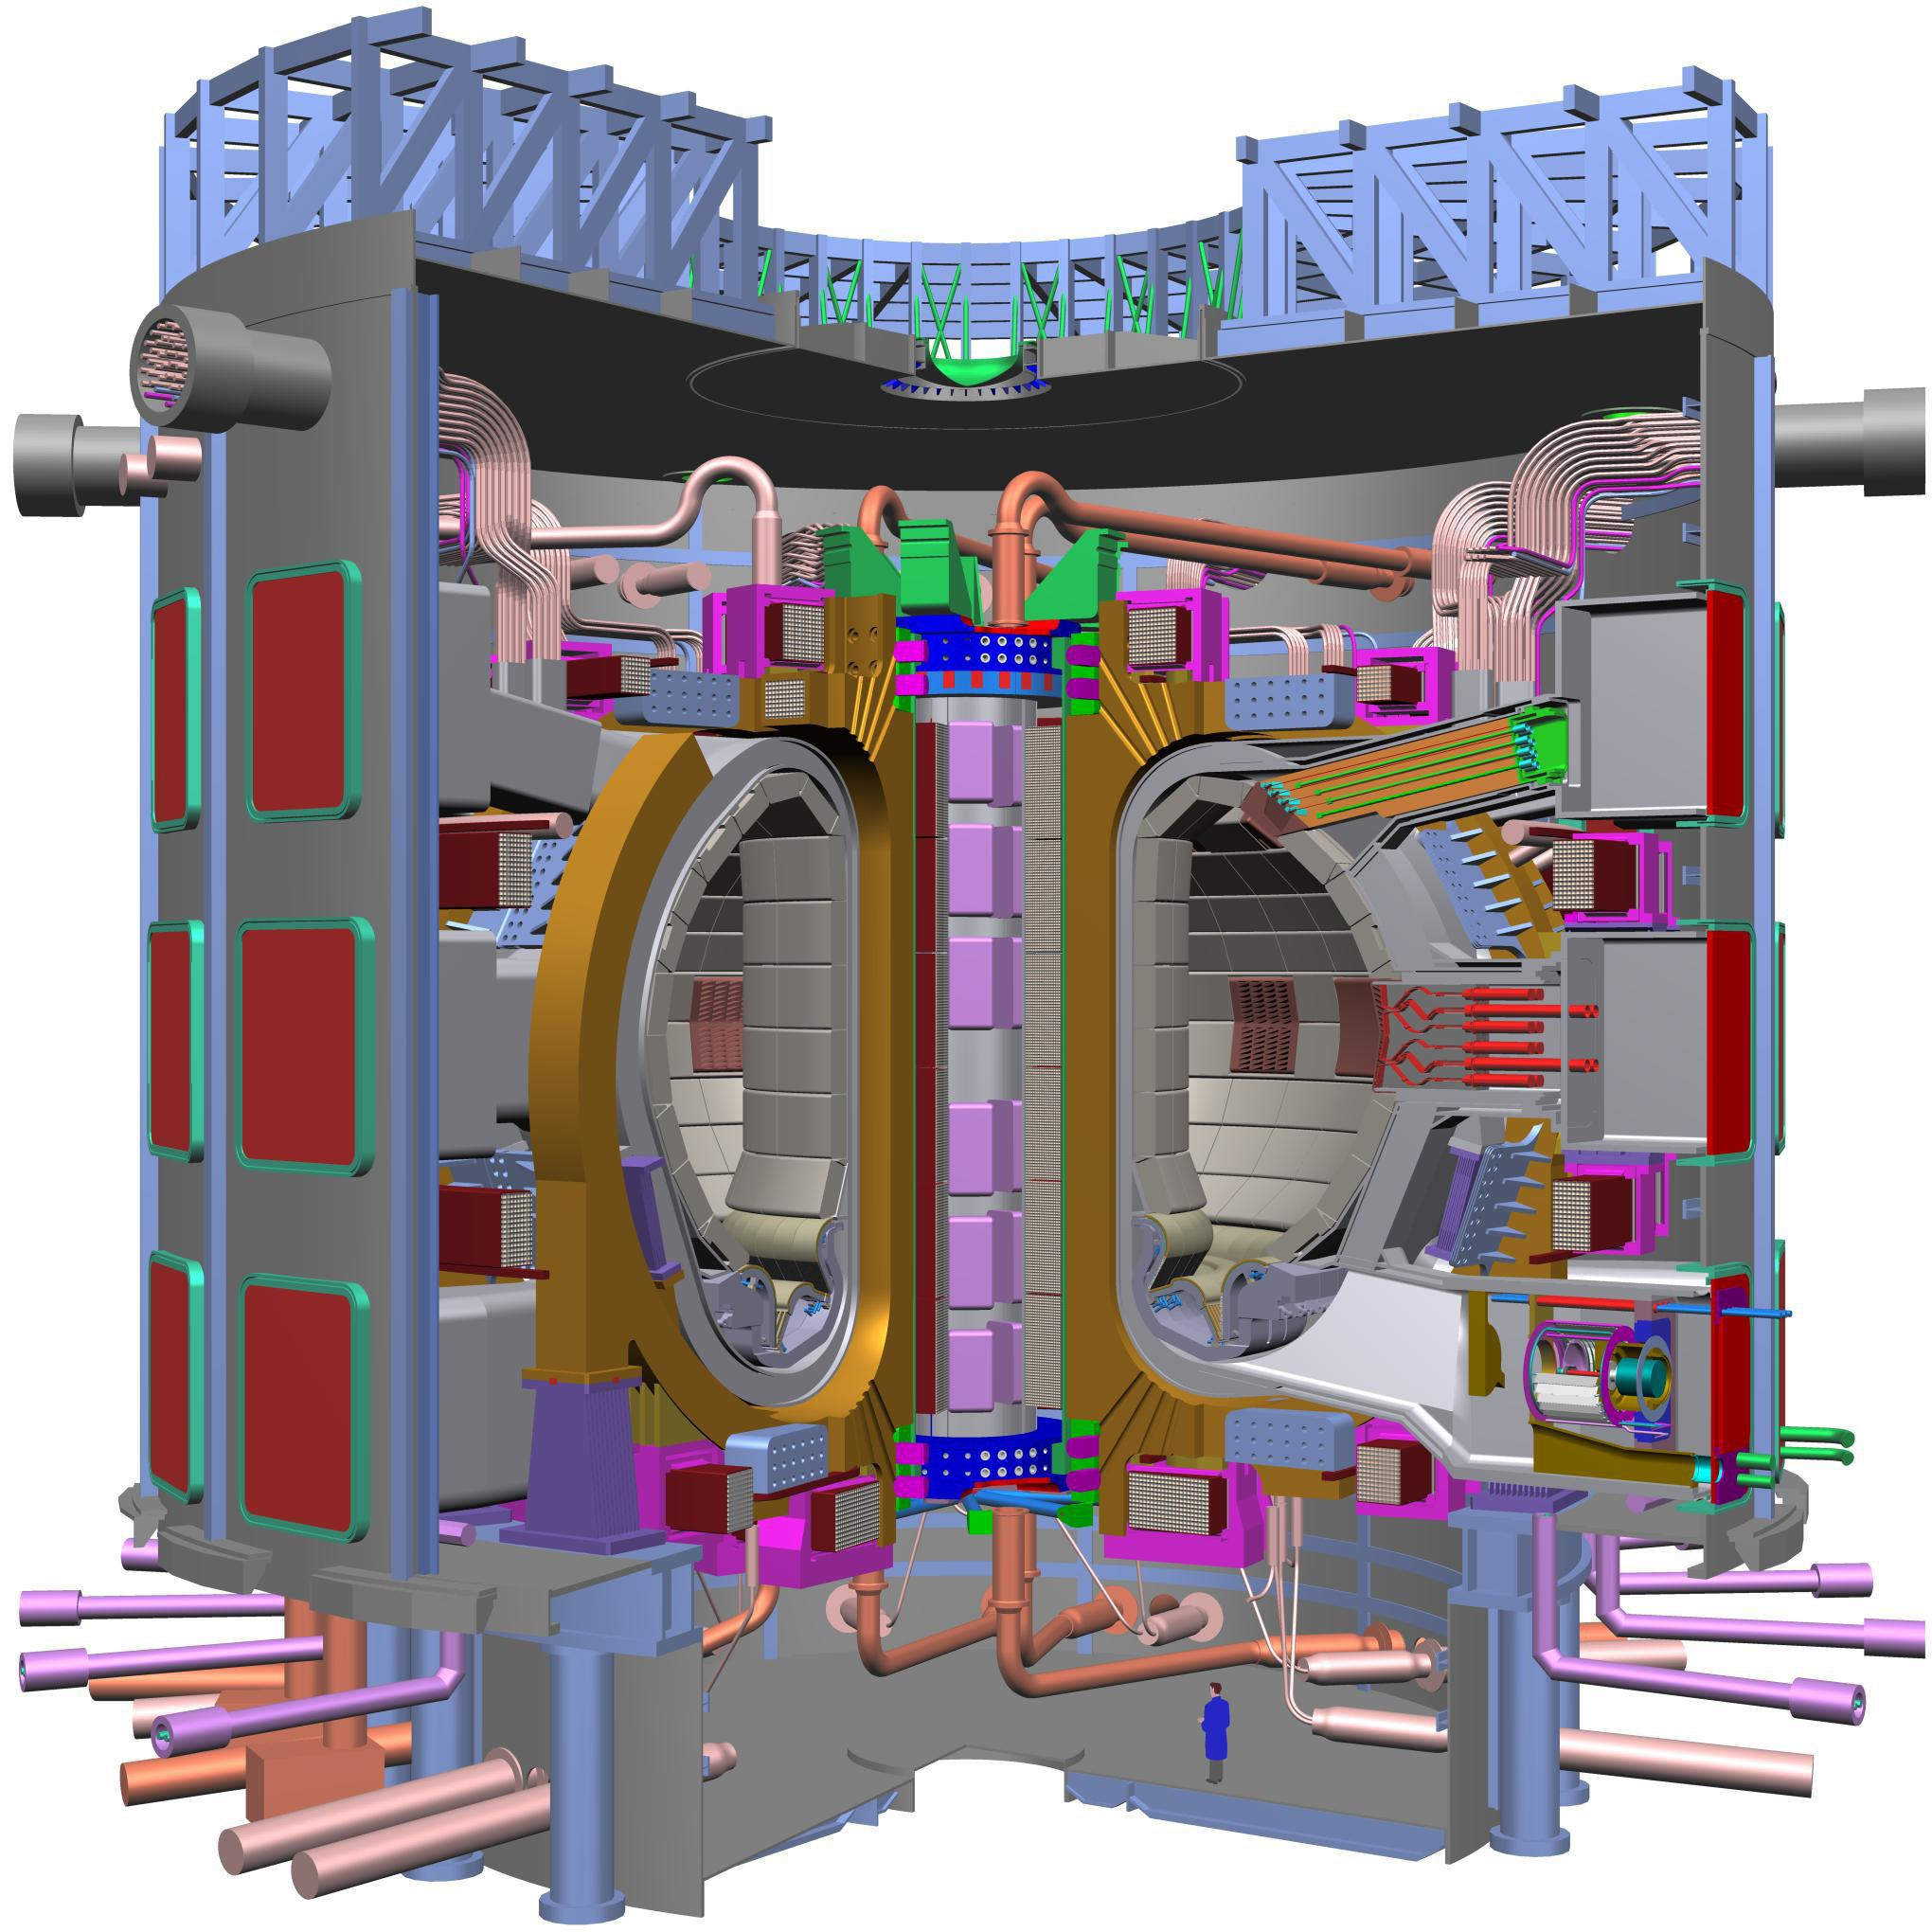
\includegraphics[width=0.8\linewidth]{iter.jpg}

{\color{gray} Iter: International Thermonuclear Experimental Reactor, Image published by U.S. Department of Energy, placed in Public Domain}}%
\only<2->{%
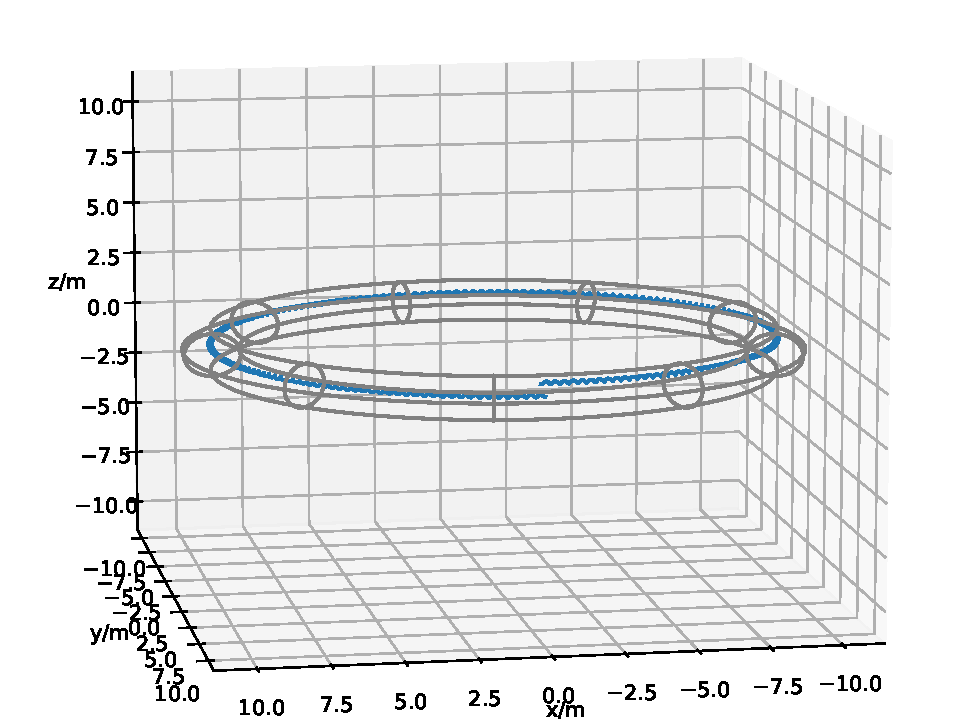
\includegraphics[width=\linewidth]{torus3_3D.pdf}}%
\end{column}
\end{columns}
\end{frame}

\begin{frame}
\frametitle{Solving the problem}
\only<1>{%
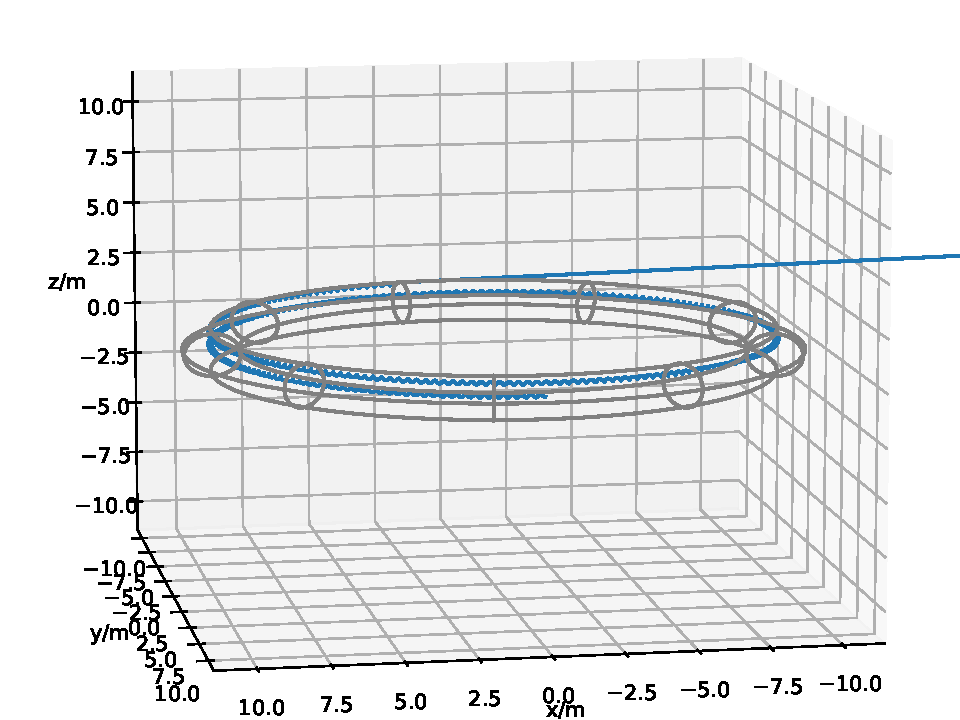
\includegraphics[width=\linewidth]{torus4_3D.pdf}
}%
\only<2>{%
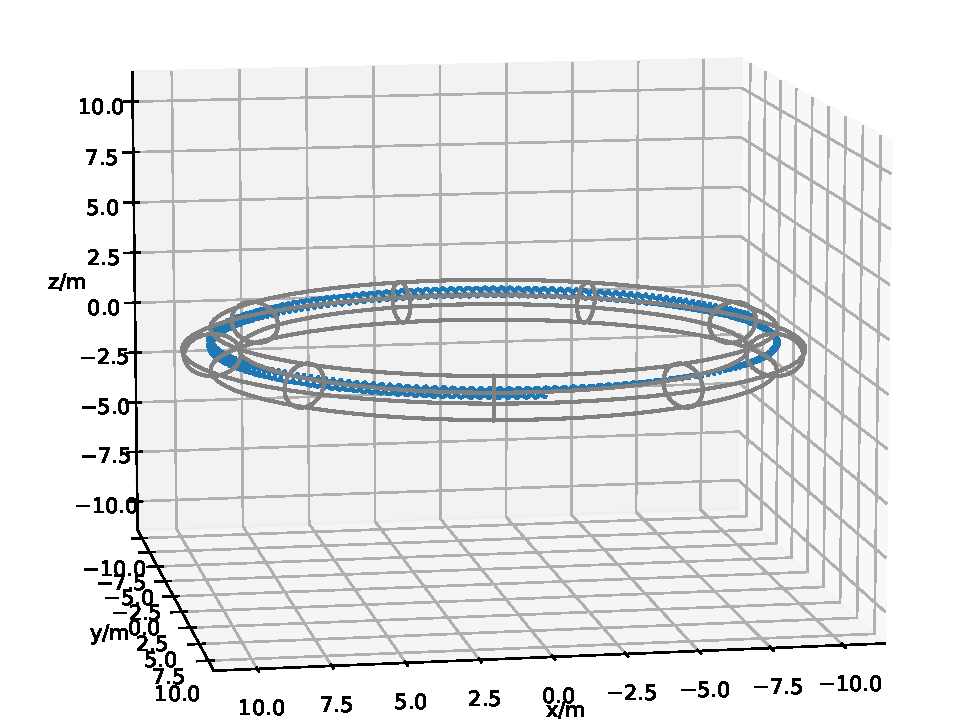
\includegraphics[width=\linewidth]{torus5_3D.pdf}
}%
\end{frame}


\begin{frame}
\begin{columns}
\begin{column}{0.5\linewidth}
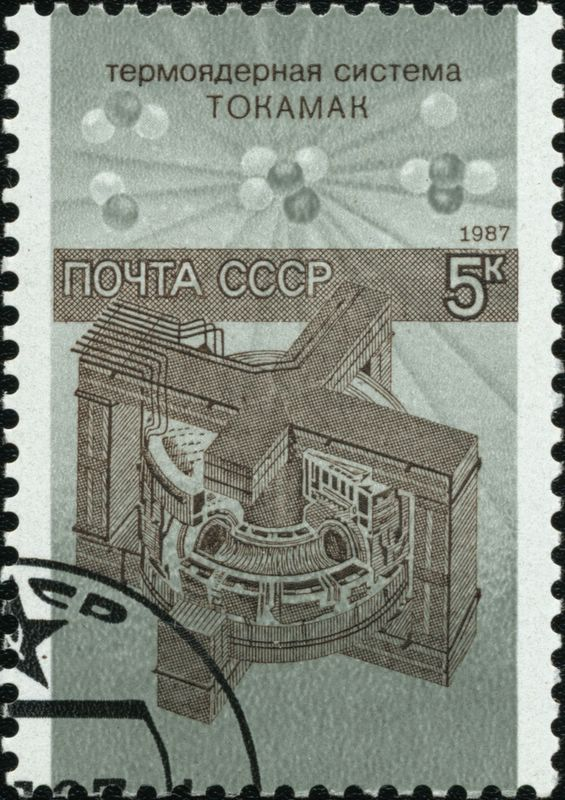
\includegraphics[width=\linewidth]{tokamak_stamp.jpg}
\end{column}
\begin{column}{0.5\linewidth}
\begin{itemize}
\item {\color{gray} Soviet Stamp from 1987 showing concept of Tokamak, Image in Public Domain}

\item <1-> Need to consider ``current" of the plasma.

\item <2-> More stabilization and control is needed.

\item <3-> Particles do follow magnetic fields!
\end{itemize}
\end{column}
\end{columns}
\end{frame}


\begin{frame}
\frametitle{Another example, Aurora}
\begin{columns}
\begin{column}{0.5\linewidth}
\begin{itemize}
\item<1-> Solar wind (ions) vs. Earth Magnetic field.


\item<2-> Why not my simulation here?

\item<3-> Here is someone elses simulation

\item<1-3> {\color{gray} Illustration originally from Nasa. Published on wikipedia, in Public Domain (Cropped to fit page) }
\end{itemize}
\end{column}
\begin{column}{0.5\linewidth}

\only<1-2>
{%
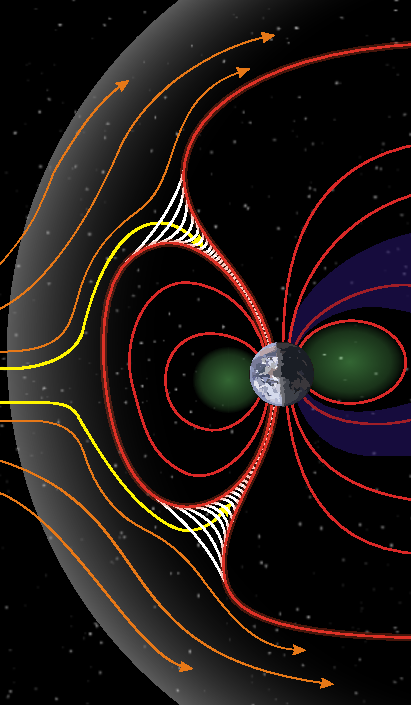
\includegraphics[width=0.8\linewidth]{Structure_of_the_magnetosphere_Nasa.pdf}%
}%
\only<3->
{
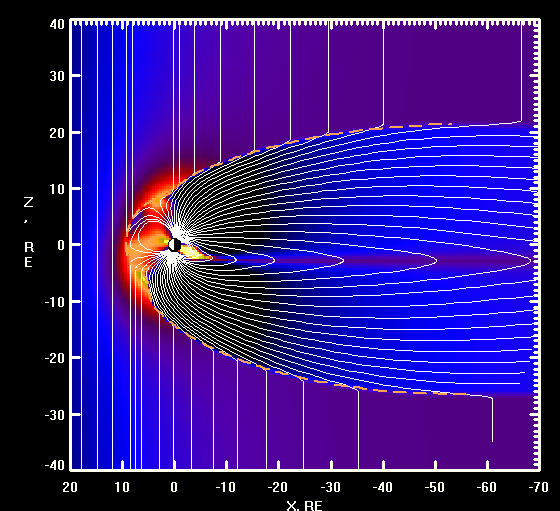
\includegraphics[width=\linewidth]{Tsyganenko1.png}
{\color{gray} Frame from animation of the Earth magnetic field during increased activity, by N. A. Tsyganenko, Published under the GNU General Public License V. 3 }
}
\end{column}
\end{columns}
\end{frame}


\begin{frame}
\frametitle{Aurora, bad simulation}

\only<1>{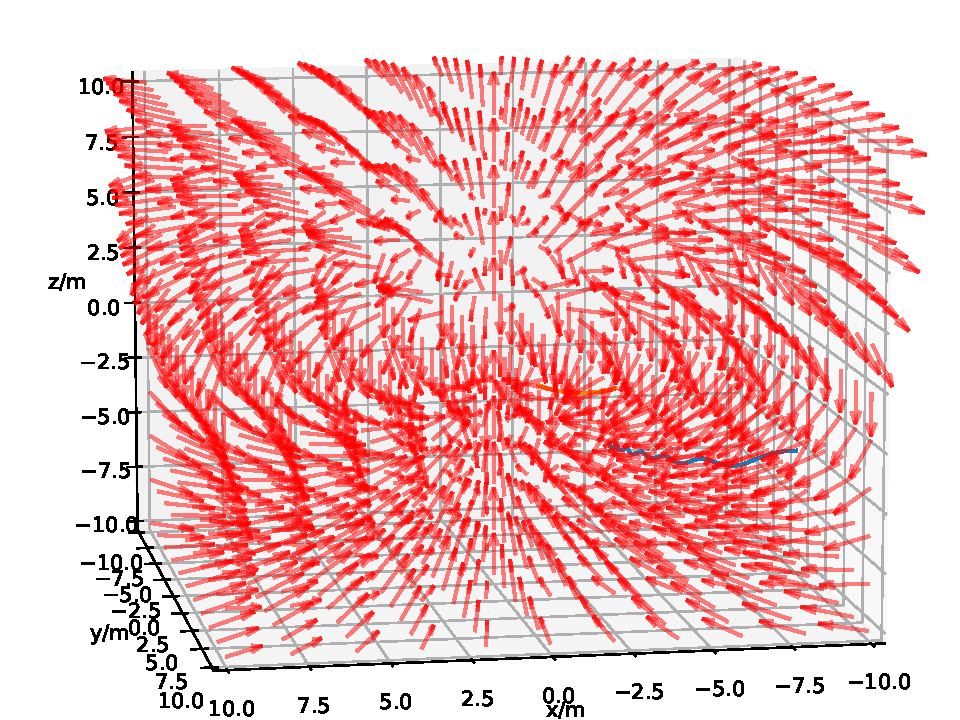
\includegraphics[width=0.8\linewidth]{dipole0.pdf}}%
\only<2>{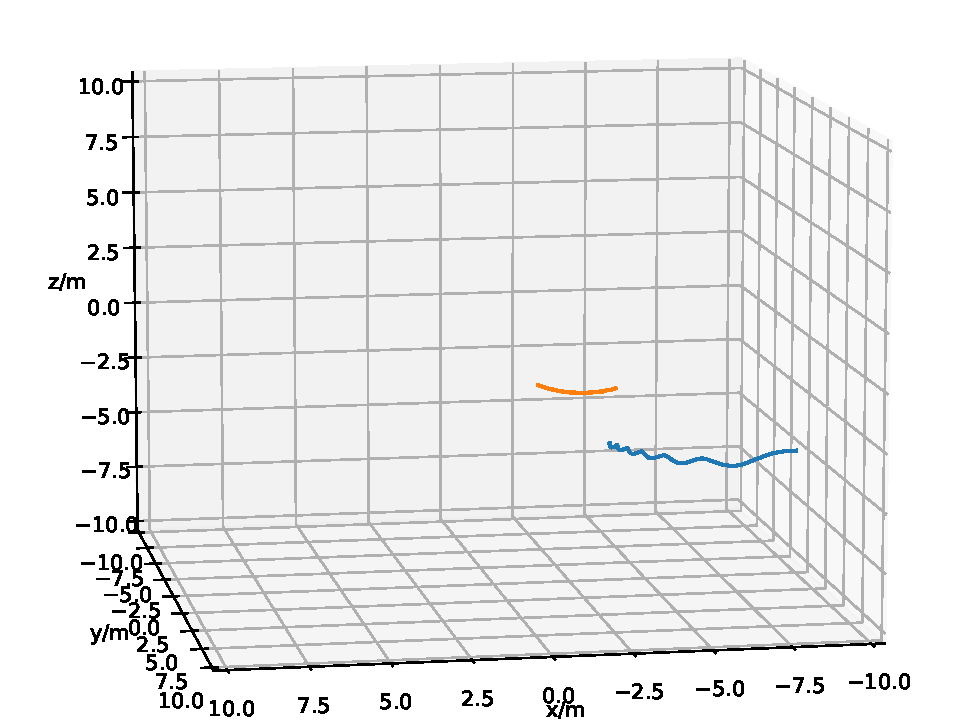
\includegraphics[width=0.8\linewidth]{dipole1.pdf}}%
\only<3>{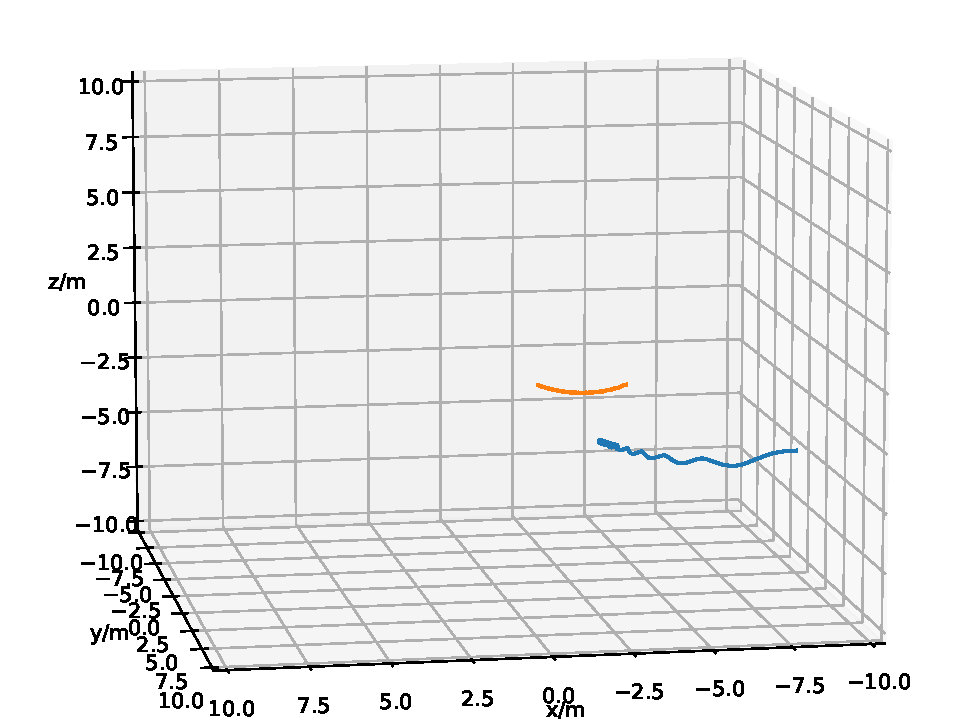
\includegraphics[width=0.8\linewidth]{dipole2.pdf}}%
\only<4>{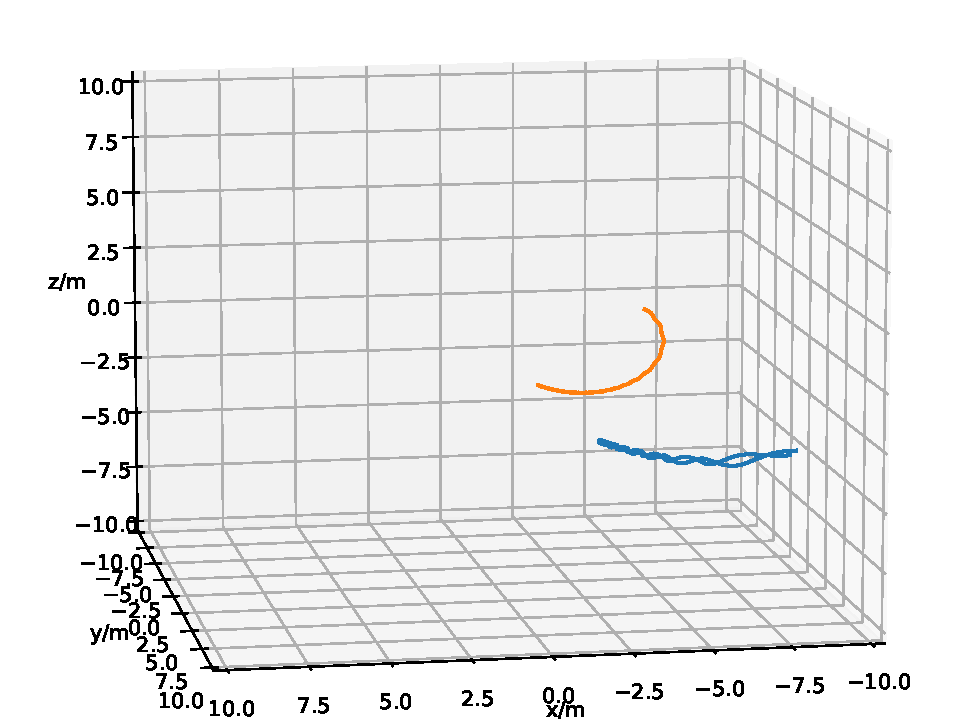
\includegraphics[width=0.8\linewidth]{dipole3.pdf}}%
\end{frame}



\section{Introducing Electric fields (10 min)}

\begin{frame}
\frametitle{Introducing Electric fields (10 min)}
\tableofcontents[currentsection]
\end{frame}


\begin{frame}
\frametitle{Electric fields}
\begin{columns}
\begin{column}{0.5\linewidth}
\begin{itemize}
\item<1-> Electric forces do work.

\item<2-> Can be used in particle accelerators.

\item<3-> Practical example, the Cyclotron.

\item<4-> Single gab, oscillating field.

\item<4-> Uses Cyclotron frequency
\end{itemize}
\end{column}
\begin{column}{0.5\linewidth}
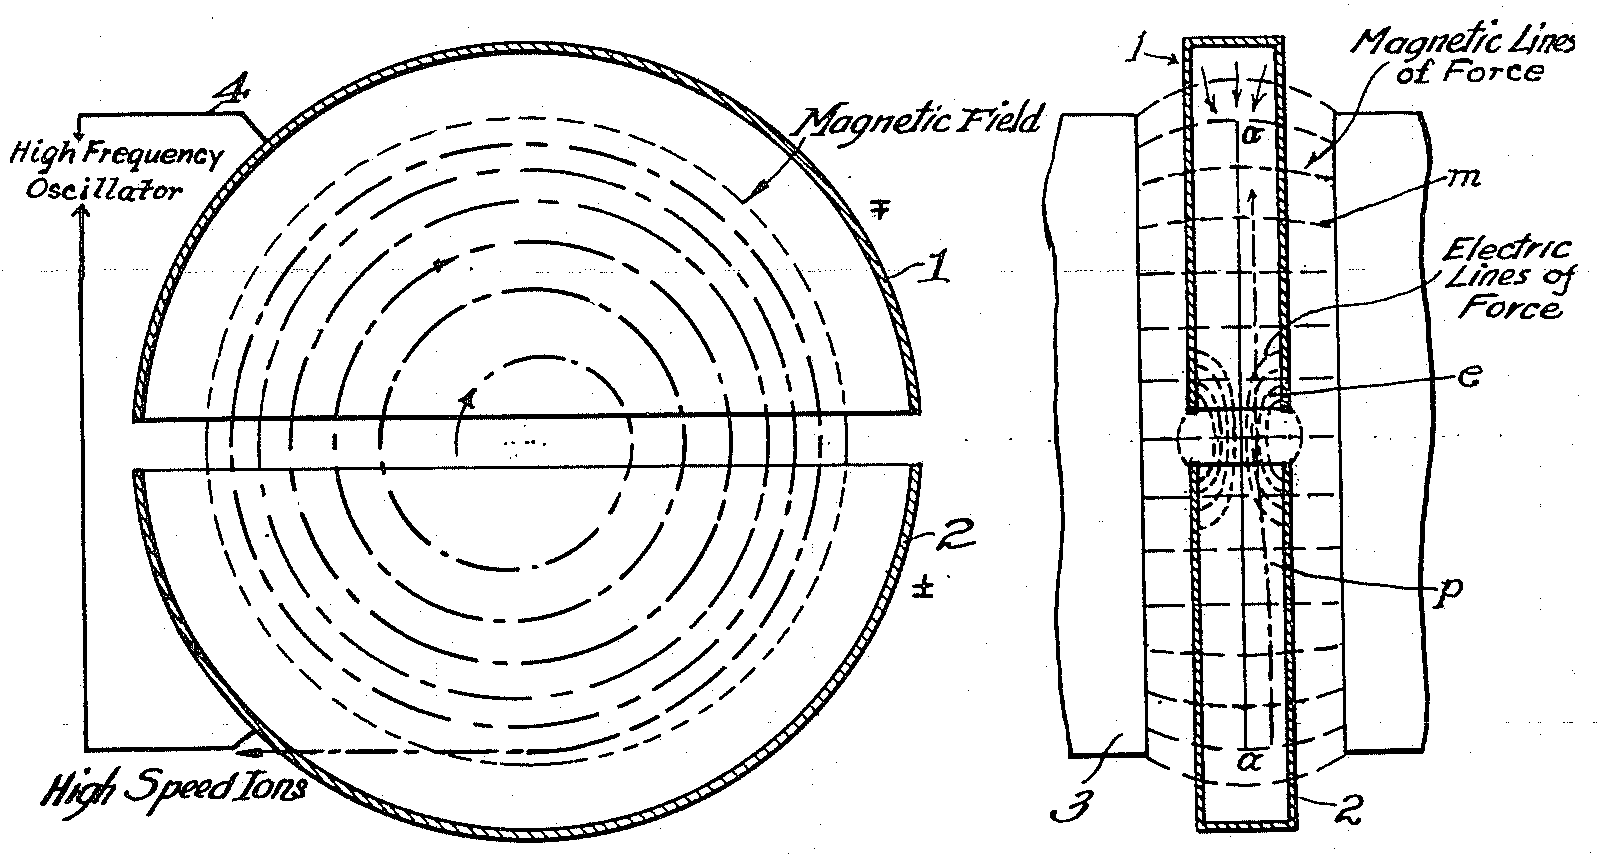
\includegraphics[width=\linewidth]{ Cyclotron_patent.png}
{\color{gray} Ernest O. Lawrence, 1934, U.S. Patent 1,948,384; image in Public Domain.}
\end{column}
\end{columns}
\end{frame}




\begin{frame}
\frametitle{Simulating the Cyclotron}
\begin{columns}
\begin{column}{0.5\linewidth}
\begin{itemize}
\item<1-> I test same $\vec{B}$ as before (around \SI{6}{\milli\tesla}), so $T\approx \SI{10}{\micro\second}$

\item<2-> $E_{max}=\SI{1}{\kilo\volt/\meter}$ (For display purposes), gab \SI{20}{\centi\meter}, radius \SI{3}{\meter}.

\item<3-> Energy depends only on the radius and $\vec{B}$ field:

\begin{equation*}
\frac{R|q|B}{m} = v_\perp
\end{equation*}


\end{itemize}
\end{column}
\begin{column}{0.5\linewidth}
\only<1>{%
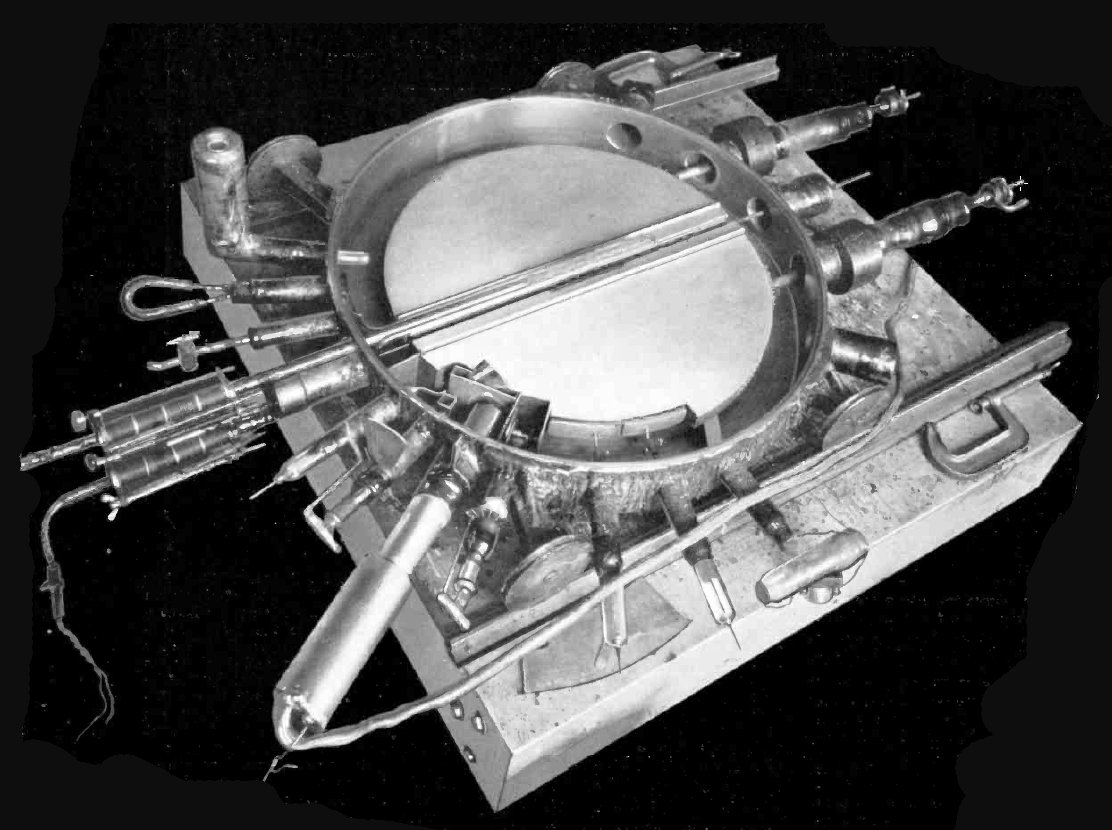
\includegraphics[width=\linewidth]{Lawrence_27_inch_cyclotron_dees_1935.jpg }
{\color{gray} Photography of Lawrence's 27-inch proof of concept Cyclotron, in Public Domain.}}%
\only<2->{%
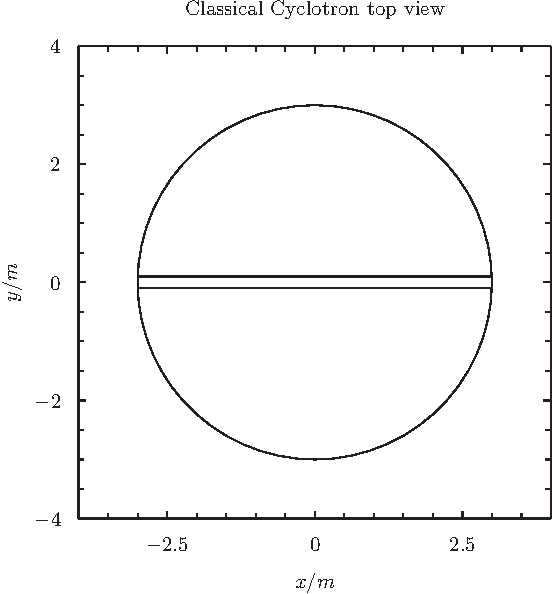
\includegraphics[width=\linewidth]{cyclotron0_xy-view.pdf}}
\end{column}
\end{columns}
\end{frame}


\begin{frame}
\only<1>{%
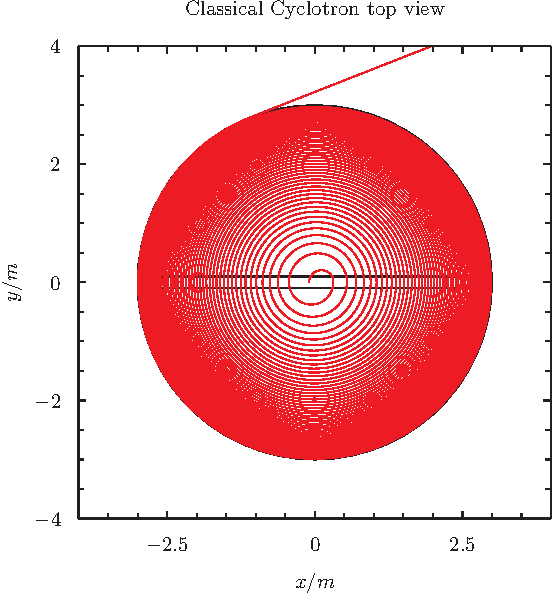
\includegraphics[width=0.8\linewidth]{cyclotron1_xy-view.pdf}}%
\only<2>{%
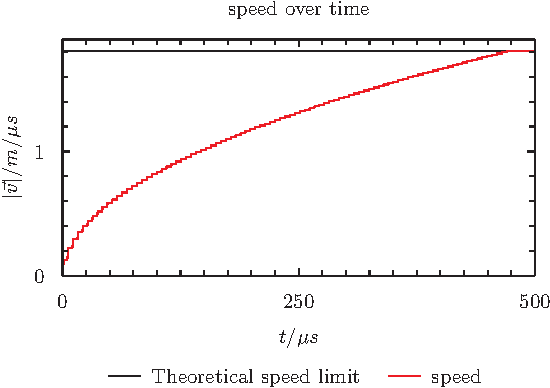
\includegraphics[width=\linewidth]{cyclotron_speed1.pdf}}%
\end{frame}


\section{Conclusion and Questions(5 min)}
\begin{frame}
\frametitle{Limitations of the Simulation}
\begin{itemize}
\item<1-> Key points changed by relativity. $\vec{v} m\rightarrow \gamma \vec{v} m$, for $\gamma=1/\sqrt{1-v^2/c^2}.$

\item<2-> $\omega_c$ depends on $r$ and $v$:

\begin{equation}
\omega_c =\frac{|q|B}{\gamma m}.
\end{equation}

\item<3-> Cyclotron needs to be synchronized.


\item<4-> Single particles is a limitations.

\item<5-> Simulating the Electric and Magnetic field would be better.
\end{itemize}
\end{frame}


\begin{frame}
\frametitle{Questions}
\end{frame}


%Electric and magnetic fields
%The Lorentz force
%Newtons 2nd law, ordinary differential equation*
%Alternative, electric and magnetic potentials

\end{document}
